%% Los cap'itulos inician con \chapter{T'itulo}, estos aparecen numerados y
%% se incluyen en el 'indice general.
%%
%% Recuerda que aqu'i ya puedes escribir acentos como: 'a, 'e, 'i, etc.
%% La letra n con tilde es: 'n.

\chapter{Metodología}
\label{metodologia}

Es sabido que tener información sobre la función de densidad de una variable aleatoria permite tener una completa descripción de la misma. Por este motivo es un problema fundamental de la Estadística obtener, a partir de la información proporcionada por una muestra,  buenas estimaciones de las funciones de densidad de una variable o vector aleatorio. 

En este sentido existen dos enfoques para abordar este problema. 

\begin{itemize}
	\item Un enfoque paramétrico: donde se considera que la función de densidad teórica pertenece a una familia de funciones de densidad $f_{X;\theta}$ conocida, indexada por el vector de parámetros $\theta$. Bajo esta suposición estimar la función de densidad teórica se reduce a estimar el valor de los parámetros del modelo a partir de la información proporcionada por la muestra. Los métodos clásicos de estimación paramétrica son: Método de los Momentos y Método de Máxima Verosimilitud. En los últimos años el Método de Logcumulantes, que se basa en la transformada de Mellin, ha ganado interés por su buena performance.
	\item Un enfoque no paramétrico: donde no se hace ninguna suposición inicial sobre la familia de densidades a las que pertenece la función de densidad teórica, sino que trata de estimarla teniendo como única información los datos muestrales, imponiendo  solamente las condiciones necesarias para que dicha estimación sea una función de densidad.
\end{itemize}

El principal aporte de esta tesis es la propuesta de un nuevo método de estimación para el parámetro de textura del modelo $\mathcal G_I^0$ con buenas propiedades que serán estudiadas a través del sesgo, del error cuadrático medio y de su capacidad para resistir presencia de datos atípicos, aún en el caso de muestras de pequeño y moderado tamaño. Este estimador surge de la minimización de distancias estocásticas entre la función de densidad teórica y una estimación no paramétrica de la función densidad subyacente utilizando núcleos asimétricos. 

En este capítulo describimos dos metodologías de estimación de la función de densidad: paramétrica y no paramétrica. Presentamos los estimadores de momentos, de Máxima Verosimilitud y Logcumulantes del parámetro de textura de la distribución $\mathcal{G}_I^0$, que son los estimadores que utilizaremos para evaluar la performance del propuesto en esta tesis. También presentamos los conceptos de estimación no paramétrica de la función de densidad, núcleos asimétricos, distancias estocásticas y estimadores de mínima distancia estocástica porque son el corazón del estimador planteado.  Asimismo hacemos una discusión de diferentes distancias estocásticas estudiadas y diferentes núcleos utilizados para estimar la función de densidad subyacente. Finalmente nuestra propuesta para estimar el parámetro de textura del modelo $\mathcal{G}_I^0$ que es el argumento que minimiza una distancia estocástica entre la función de densidad teórica del modelo teórico y una estimación no paramétrica de la función de densidad subyacente. 


\section{Estimación Paramétrica}
\label{EstimacionParamétrica}

Esta metodología de estimación propone, a partir del conocimiento de la familia de densidades a la que pertenece la función de densidad teórica, estimar los parámetros que caracterizan dicha función de densidad a partir de datos muestrales. A continuación presentaremos métodos clásicos de estimación paramétrica.

\subsection{Método de los Momentos}
\label{MetodoMOM}
El Método de los Momentos (MOM) fue introducido por Karl Pearson en el año 1894 y se basa en la idea intuitiva de pensar que, si los datos muestrales provienen de una determinada distribución de probabilidad, entonces los momentos muestrales deberían dar buenas estimaciones de los correspondientes momentos poblacionales. 

\begin{definition}
Si $X_1, \ldots, X_n$ es una muestra de variables aleatorias independientes e idénticamente distribuidas con función de densidad $f_{X;\theta}$, donde $\theta \in \mathbb{R}$ es el parámetro a estimar, y $g(x)$ una función de $\mathbb{R}$ en $\mathbb{R}$, el Método de los Momentos propone como estimador $\hat{\theta}_{\text{mom}}$ de $\theta$ aquel valor del parámetro que es solución de la ecuación  $\dfrac{1}{n} \sum_{i=1}^n g(X_i)=E_{\theta}(g(X_i)).$  
Si en cambio $X_i \sim f_{X;\theta}$ con $\theta \in \Theta \subset \mathbb{R}^k$, entonces $\hat{\theta}_{\text{mom}}$ será el valor $\theta$ que verifica el sistema de ecuaciones $\dfrac{1}{n} \sum_{i=1}^n g_s(X_i)=E_{\theta}(g_s(X_i))$ donde $s=1, \ldots k$ y $g_s(x)$ son $k$ funciones de $\mathbb{R}$ en $\mathbb{R}$.
\end{definition}


Obsevemos que si $g_s(x)=x^s$ la definición es consistente con la idea intuitiva mencionada anteriormente.
%Entonces, si $g(x)=x$ y el correspondiente momento muestral es $m_k=\dfrac{\sum_{i=1}^n X_i^k}{n}$. Entonces, si $X_1, \ldots X_n$ es una muestra de variables aleatorias independientes e idénticamente distribuidas 
%
%Recordemos que el $k$-ésimo momento muestral de una variable aleatoria $X$, tomado alrededor del origen, es $M_k=E(X^k)$.

El estimador por Momentos Fracionales ha sido estudiado en los últimos tiempos. \citet{Frery97} utilizaron este método para estimar los parámetros de la distribución $\mathcal{G}_A^0(\alpha,\gamma,L)$ con $L$ conocido,  \citet{GambiniSC08} aplicaron este método para el problema de detección de bordes en imágenes SAR. En esta tesis se utilizarán los momentos de orden $1$ y de orden $\frac{1}{2}$ ya que estos momentos existen para valores de $\alpha<-1$.

Las ecuaciones de momento de orden $1$ y de orden $\frac{1}{2}$ para estimar los parámetros de la distribución $\mathcal G_I^0$ son:

\begin{align}
\label{momento1medio}
\nonumber \overline{X}=&\dfrac{\gamma}{-\alpha - 1}, \\
\nonumber \\ 
\dfrac{\sum_{i=1}^n X_i^{1/2}}{n}=&\dfrac{\gamma^{1/2}}{L^{1/2}}\dfrac{\Gamma(-\alpha - 1/2)}{\Gamma(-\alpha)}\dfrac{\Gamma(L+ 1/2)}{\Gamma(L)}.
\end{align}


\subsection{Método de Máxima Verosimilitud}
\label{MetodoMV}


El Método de Máxima Verosimilitud (MV) fue popularizado por Sir Ronald Fisher entre 1912 y 1922. Sin embargo este método había sido utilizado antes por Gauss, Laplace entre otros investigadores. 
La idea del método consiste en, dada una muestra, estimar los parámetros de la distribución que maximice la credibilidad de que haya salido esa muestra. 
Esto requiere mirar a la función de densidad conjunta como función de los parámetros, a esta función se llama función de verosimilitud.

\begin{definition}
Si $X_1, \ldots, X_n$ es una muestra de variables aleatorias independientes e idénticamente distribuidas con función de densidad $f_{X;\theta}$  con $\theta \in \Theta \subset \mathbb{R}^k$, diremos que $\widehat{\theta}_{\text{MV}}$ es el estimador de Máxima Verosimilitud de $\theta$ si verifica que 
\begin{align}
\widehat{\theta}_{{\text{\tiny{\text{MV}}}}}=\arg\max_{\vec{\theta} \in \Theta} L(\theta \mid \vec{X}=\vec{x}),
\end{align}
siendo $L(\theta \mid \vec{X}=\vec{x})$ la función de verosimilitud, que es la función de densidad conjunta del vector aleatorio $\vec{X}$ mirada como función del vector de parámetros $\theta$, sabiendo que salió la muestra $\vec{x}$.
\end{definition}
Este estimador tiene muy buenas propiedades asintóticas, éstas se pueden encontrar en  \citet{Casela2002}. 
Además de ser consistente, este estimador es asintóticamente normal y eficiente bajo ciertas condiciones de regularidad.

El parámetro $\gamma$ en la distribución $\mathcal{G}_I^0$  es proporcional al brillo y es un parámetro de escala. Con el fin de reducir nuestro análisis a un solo parámetro, y con el propósito de hacer los resultados comparables, basamos nuestro análisis en la condición $E(Z)=1$ que vincula la textura con el brillo. Esta condición nos da una relación entre $\gamma$ y $\alpha$ que es la siguiente:
\begin{align}
\label{gama*}
\gamma=-\alpha-1. 
\end{align}
A este valor de $\gamma$ lo llamaremos $\gamma^*$.

Entonces, si $Z_1,\ldots Z_n$ una muestra de variables aleatorias independientes e idénticamente distribuidas donde 
%%% ACF Mejor usá \gamma^*, y ¿no te olvidaste de L?
$Z_i \sim f_{\mathcal G_I^0(\alpha,-\alpha-1)}(z)$,  el logaritmo de la función de verosimilitud bajo la condición~\eqref{gama*} es:
\begin{align}
\nonumber \log (L(\alpha) \mid \vec{Z}=\vec{z})&=n(L \log L+\log \Gamma(L-\alpha)-\log \Gamma(-\alpha) -\alpha \log(-\alpha-1))\\
& + (L-1) \sum_{i=1}^n \log(z_i)-(L-\alpha) \sum_{i=1}^n\log(-\alpha-1+z_i L).
\end{align}


Por lo tanto, el estimador de Máxima Verosimilitud (MV) del parámetro de textura es:
%%% ACF No sería bueno poner el espacio de búsqueda de \alpha?
\begin{align}
\widehat{\alpha}_{{\text{\tiny{MV}}}}=\arg\max_{\alpha} \log(L(\alpha)\mid \vec{Z}=\vec{z}).
\end{align}

Algunos autores evaluaron la performance del estimador de Máxima Verosimilitud del parámetro de textura del modelo  $\mathcal G_I^0$. \citet{VasconcellosFrerySilva:CompStat} cuantificaron el sesgo de este estimador y propusieron una corrección de segundo orden de acuerdo a \citet{cox1968}. 
\citet{CribariFrerySilva:CSDA} desarrollaron una corrección del sesgo de $\widehat{\alpha}_{\text{{\text{\tiny{MV}}}}}$ del modelo $\mathcal G^0_A$ usando técnicas de remuestreo a expensas de un alto costo computacional.

En la figura~\ref{MV} se muestra el gráfico del logaritmo de la función de verosimilitud en función de $\alpha$, para distintos tamaños de muestra $n$ y para dos valores del parámetro de textura: $\alpha=-1.5$ y $\alpha=-5$ para el caso de $L=3$. Se puede observar que, para zonas extremadamente texturadas la función de verosimilitud muestra claramente un máximo. Sin embargo, para el caso de zonas texturadas esta función es bastante plana, incluso podría ser monótona dependiendo de la muestra. Esto puede originar problemas numéricos al momento de encontrar el máximo.  

\begin{figure}[hbt]
	\centering    
	\subfigure[$\alpha=-1.5$]{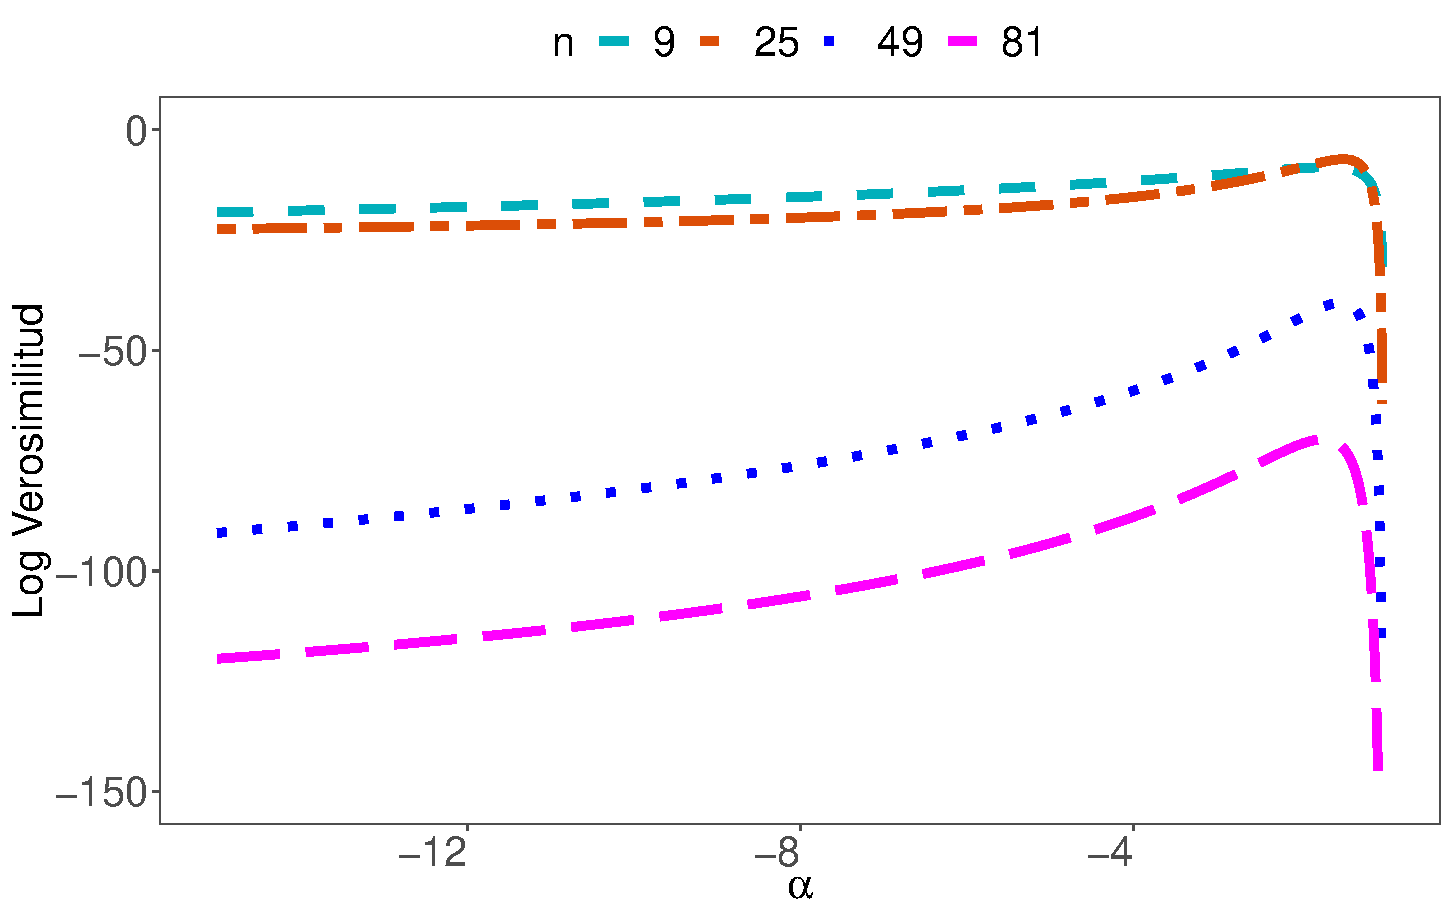
\includegraphics[width=.46\linewidth]{../../Figures/Tesis/Capitulo5/Verosimilitud1punto5_2.pdf}} \qquad
	\subfigure[$\alpha=-5$]{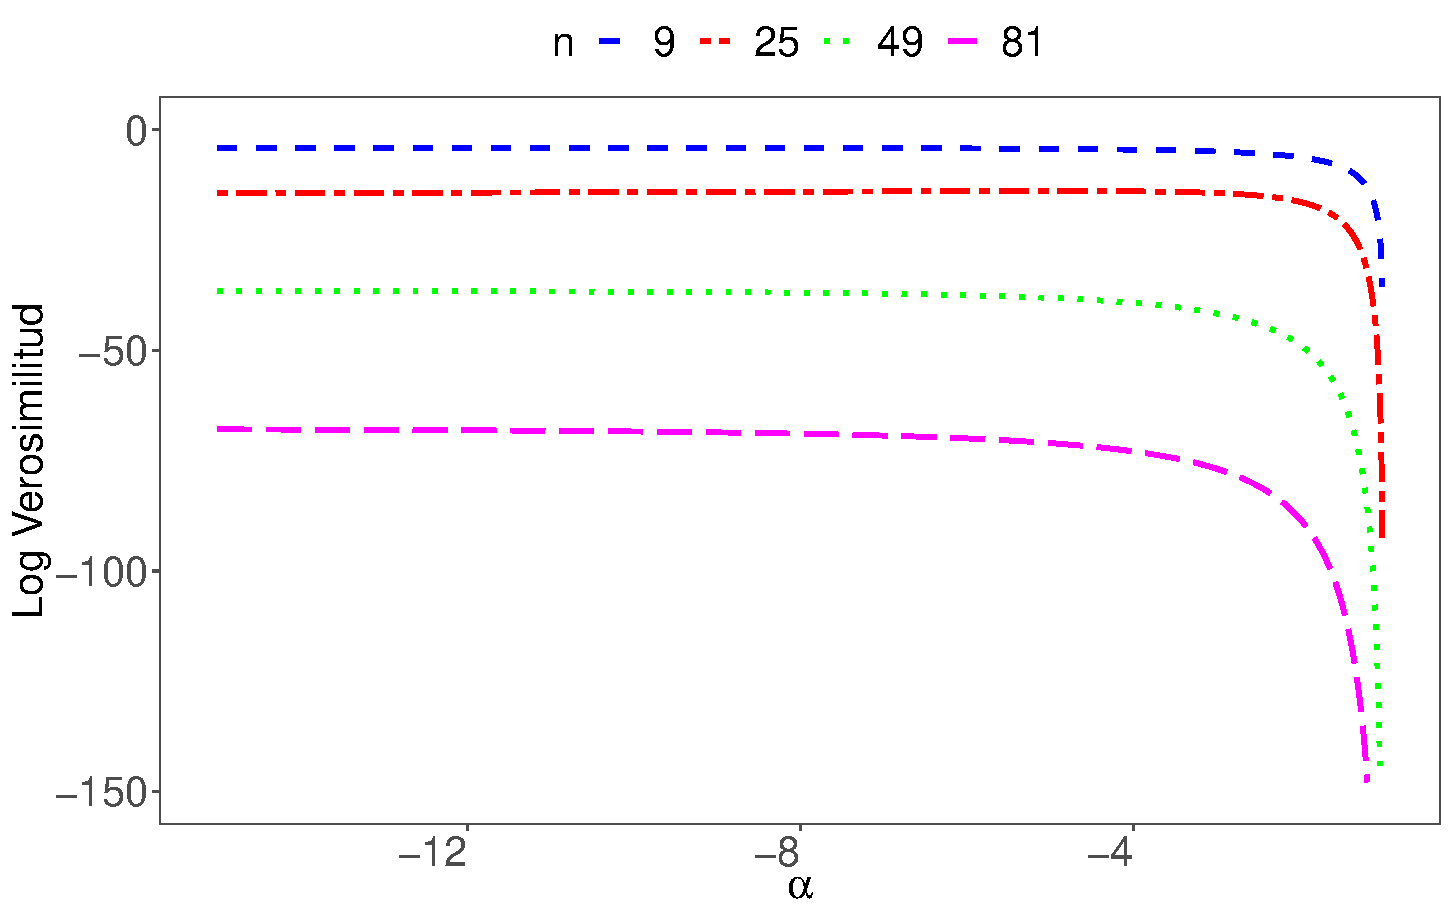
\includegraphics[width=.46\linewidth]{../../Figures/Tesis/Capitulo5/Verosimilitud-5_2.pdf}}
	\caption{\label{MV} Función de verosimilitud para $L=3$}
\end{figure}

También se podría encontrar $\widehat{\alpha}_{{\text{\tiny{MV}}}}$ como la solución de la siguiente ecuación no lineal.
\begin{align}
\label{rootML}
\Psi^0(-\widehat{\alpha}_{{\text{\tiny{MV}}}})-\Psi^0(L-\widehat{\alpha}_{{\text{\tiny{MV}}}})-\log(-1-\widehat{\alpha}_{{\text{\tiny{MV}}}})+{} \nonumber\\
\frac{\widehat{\alpha}_{{\text{\tiny{MV}}}}}{-1-\widehat{\alpha}_{{\text{\tiny{MV}}}}}+
\frac{1}{n}\sum_{i=1}^n{\log(-1-\widehat{\alpha}_{{\text{\tiny{MV}}}}+Lz_i)}-{}
\nonumber
\\ \frac{\widehat{\alpha}_{{\text{\tiny{MV}}}}-L}{n}\sum_{i=1}^n \frac1{-1-\widehat{\alpha}_{{\text{\tiny{MV}}}}+Lz_i}= 0, 
\end{align}
donde $\Psi^0(\cdot)$ es la función digamma. Este sistema no tiene una solución analítica cerrada, por lo tanto es necesario la utilización de rutinas numéricas para encontrar dicha solución que puede incluso no existir.

\subsection{Logmomentos y Logcumulantes}
\label{MetodoLC}

Es conocida la relación que existe entre los momentos y la función característica de una variable aleatoria con la transformada de Fourier de su función de densidad. 

\begin{definition}
Si $X$ es una variable aleatoria continua con función de densidad $f_X(x)$, la función característica $\phi_X: \mathbb{R} \rightarrow \mathbb{C}$ se define como 
\begin{align}
\phi_X(t)=E(e^{itX})=\int_{-\infty}^{\infty} e^{itx} f_X(x) dx = \mathcal{F}\{f_X\}(t),
\label{fi_caracteristica}
\end{align}
siendo $\mathcal{F}\{f_X\}$ la transformada de Fourier de $f_X$.
\end{definition}

Cuando los momentos de orden $k$ de una variable aleatoria existen, es decir, cuando $E(X^k)< \infty$, se puede apelar a la relación~\eqref{fi_k} para calcular dichos momentos. Entonces
\begin{align}
\phi_X^{(k)}(0)=i^k E(X^k),
\label{fi_k}
\end{align}
con $\phi_X^{(k)}$ la derivada de orden $k$ de $\phi_X$ evaluada en $t=0$. Luego, los momentos de orden $k$ se pueden definir como 
\begin{align}
\label{MomentosPrimerTipo}
m_k=E(X^k)=i^{-k} \phi_X^{(k)}(t)\big\arrowvert _{t=0}\cdot
\end{align}

Si llamamos $\psi_X=\log(\phi_X)$, los cumulantes de orden $k$ se definen como 
\begin{align}
\label{CumulantePrimerTipo}
\kappa_k=i^{-k} \psi_X^{(k)}\big\arrowvert _{t=0}\cdot
\end{align}

 \citet{nicolas2002} proponen utilizar la transformada de Mellin en lugar de la transformada de Fourier en~\eqref{fi_caracteristica}, para el caso donde la función de densidad $f_X$ de la variable aleatoria $X$ tiene soporte positivo. De esta manera surgen nuevas características para la variable aleatoria que son los Logmomentos (MomL) y los  Logcumulantes (LC). Los autores proponen llamar a esta metodología Estadísticas de Segundo Tipo. Entonces definen:
\begin{itemize}
\item Primera función característica de segundo tipo.
	\begin{align}
	\Phi_X(s)=\int_{0}^{\infty} x^{s-1} f_X(x) dx = \mathcal{M}\{f_X\}(s)\cdot
	\label{PrimerFuncionCaract}
	\end{align}
\item Momentos de segundo tipo.
	\begin{align}
	\label{MomentoSegundoTipo}
	\tilde{m}_k=\Phi_X^{(k)}(s) \big\arrowvert _{s=1}\cdot
	\end{align}


Una propiedad interesante que cumplen las derivadas de orden $k$ de la transformada de Mellin de una función $h(x)$ es $\mathcal{M}\{\ln(x)^k h(x)\}(s)=\mathcal{M}^{(k)}\{h(x)\}(s)$. Entonces, aplicando esta propiedad a~\eqref{PrimerFuncionCaract} y~\eqref{MomentoSegundoTipo}, y considerando $h=f_X$ se obtiene:
	\begin{align}
	\label{MomL}
	\nonumber \tilde{m}_k&=\Phi_X^{(k)}(s) \big\arrowvert _{s=1} =\mathcal{M}^{(k)}\{f(x)\}(s) =\mathcal{M}\{f(x) \log(x)^k\}(s)\big\arrowvert _{s=1}          \\
 	        &=\int_{0}^{\infty} \log(x)^k f_X(x) dx \cdot
	\end{align}

	Esta última ecuación sugiere llamar a los momentos de segundo tipo como Logmomentos (MomL).
	
\item Segunda función característica de segundo tipo.

      Manteniendo la analogía con las estadísticas de primer tipo, \citet{nicolas2002} definen la \textit{Segunda función característica de segundo tipo} como
      \begin{align}
      \label{Sgunda Psi}
      \Psi_X(s)=\log(\Phi_X)(s).
      \end{align}
      
\item Cumulantes de segundo tipo.

	  Se definen como los cumulantes de segundo tipo las derivadas de orden $k$ de la segunda función característica de segundo tipo, evaluadas en $s=1$. Entonces,
	  \begin{align}
	  \label{CumulanteSegundoTipo}
	  \tilde{\kappa}_k=\Psi_X^{(k)}\big\arrowvert _{s=1}.
	  \end{align}
	  
Como en el caso de MomL, los cumulantes de segundo tipo se llamarán Logcumulantes (LC).
\end{itemize}

Para el caso donde $f_X(u) = \mathcal{G}_I^0(u)$ se obtiene:
	\begin{align}
	\Phi_X(s) &= \dfrac{\left(\frac{L}{\gamma}\right)^{1-s}\Gamma(-1+L+s)\Gamma(1-s-\alpha)}{\Gamma(L)\Gamma(-\alpha)} \\
	\vspace{1cm}
	\nonumber \widetilde{m}_1 &=  \frac{d \Phi_X(s)}{ds } \big\arrowvert _{s=1}\\
					& = -\log\left(\frac{L}{\gamma}\right) + \Psi^0(L) - \Psi^0(-\alpha).
	\end{align}

Usando los desarrollos presentados en \citet{Tison2004} tenemos que $\widetilde{k}_1 = \widetilde{m_1}$. Por lo tanto 
\begin{align}
\label{MomLC}
\widetilde{k}_1 =   -\log \left(\frac{L}{\gamma}\right) + \Psi^0(L) - \Psi^0(-\alpha).
\end{align}

Además, si $Z_1,\ldots,Z_n$ es una muestra de variables aleatorias independientes e idénticamente distribuidas donde $Z_i \sim \mathcal{G}_I^0$, usando\eqref{MomL} tenemos que LC es
\begin{align}
\label{EstimadorMomLC}
\widehat{\widetilde{k}}_1 =\dfrac{1}{n} \sum_{i=1}^k\log z_i\cdot
\end{align}

Asumiendo que vale la relación~\eqref{gama*}, $\gamma^*=-\alpha-1$, el estimador Logcumulantes del parámetro de textura $\alpha$ de la distribución $\mathcal{G}_I^0$, que lo llamaremos $\widehat\alpha_{\text{\tiny{LC}}}$, es la solución de la ecuación    
\begin{align}
\widehat{\widetilde{k}}_1 =   -\log \frac{L}{-\alpha-1} + \Psi^0(L) - \Psi^0(-\alpha),
\end{align}
es decir, la solución de la ecuación
\begin{equation} \label{eq:logm}
\frac{1}{n} \sum_{i=1}^n\log z_i =   -\log \frac{L}{-\alpha-1} + \Psi^0(L) + \Psi^0(-\alpha).
\end{equation}


\section{Estimación No Paramétrica}

Como mencionamos anteriormente, otra posibilidad para estimar los parámetros de la función de densidad de una variable aleatoria es la estimación no paramétrica. Esta metodología de estimación  no determina a priori ningún modelo para la distribución de la variable aleatoria de interés, y propone estimadores de la función de densidad sin más límites que los necesarios para que estos estimadores cumplan con las condiciones de ser una función de densidad.


\subsection{Núcleos}
Estimar una función de densidad desconocida a partir de datos muestrales es un problema clásico en estadística. Si se conoce la familia de distribuciones de donde proviene la muestra, se puede dar una estimación de los parámetros de la función de densidad subyacente usando la metodología presentada en la sección~\ref{EstimacionParamétrica}. 

Otra forma de abordar el problema de la estimación de la función de densidad subyacente $f$ es a través de una estimación no paramétrica de la misma. El más sencillo y más conocido de estos estimadores es el histograma. De acuerdo a \citet{Scott1992} el histograma está determinado por la muestra ${x_1, \ldots, x_k}$ y por la partición ${t_k, -\infty<j<+\infty}$ de la recta. Sea $B_k=[t_k,t_{k+1})$  el $k$ ésimo intervalo, y supongamos que $t_{k+1}-t_k=h$ para todo $k$. Entonces el estimador $\widehat{f}_\text{h}$ de $f$ se define como 

\begin{align}
\widehat{f}_{\text{h}}(x)=\frac{1}{n h} \sum_{i=1}^n I_{\text{B}_i} (x_i)=\dfrac{N_i}{n h} \text{ para } x \in B_i,
\end{align}
donde $h$ es la longitud de los intervalos $B_i$ que suponemos la misma, $N_i$ la cantidad de observaciones muestrales que caen dentro del intervalo $B_i$ e $I_{B_i}(x)$ es la función indicadora definida en $B_i$. En el caso donde los intervalos tienen distinta longitud se deberá dividir por la longitud de cada uno dentro de la sumatoria.

Este estimador es muy utilizado especialmente cuando se quiere hacer un estudio exploratorio de la distribución de los datos, pero provee una estimación de la función de densidad que no es continua y, por lo tanto, no derivable. Estas propiedades son deseables, principalmente cuando se trabaja con variables aleatorias continuas.

\subsubsection{Núcleos simétricos}
\citet{Rosenblatt56} y \citet{Parzen62} avanzaron en la búsqueda de un estimador para $f$ y propusieron los estimadores tipo núcleo, con núcleo simétrico. Si consideramos $X_1,\ldots,X_n$ una muestra de variables aleatorias independientes e idénticamente distribuidas este estimador se define como
\begin{align}
\label{KS}
\widehat{f}_{\text{\tiny{S}}_n}(x)=\frac{1}{n b} \sum_{i=1}^n K \left(\dfrac{x-X_i}{b}\right),
\end{align}
donde $b$ es el parámetro de suavizamiento llamado también ``ancho de banda'', y $K(x)$ es una función llamada ``núcleo'' que generalmente es una función de densidad simétrica y satisface ciertas condiciones de regularidad. Estos estimadores fueron muy estudiados por diversos autores; en \citet{Silverman1986} y en \citet{Scott1992} se puede ver un exhaustivo estudio de ellos y sus propiedades. 
En particular, se puede mostrar que estos estimadores son consistentes en cada $x$ si se cumple que  
\begin{align}
\label{nh}
b \to 0,  \quad nb \to +\infty \text{ cuando } n \to +\infty
%\lim\limits_{n\to\infty} b_n=\infty \text{ y } \lim\limits_{n\to\infty} nb_n=\infty.
\end{align}	

Asimismo se pueden obtener expresiones para el sesgo y la varianza:
\begin{align}
\label{SesgoVar}
B(\widehat{f}_{\text{\tiny{S}}_n}(x))=\dfrac{b^2 f''(x) k_2}{2}+O(b^4), \text{ y}\\
Var(\widehat{f}_{\text{\tiny{S}}_n}(x))\approx \dfrac{1}{nb} \int_{-\infty}^{\infty} K^2(t)dt,
\end{align}	
respectivamente, donde $k_2=\displaystyle{\int_{-\infty}^{\infty}} x^2 K(x)dx$. Esto muestra el compromiso que existe entre el sesgo y la varianza, una rápida convergencia a $0$ del parámetro $b$ genera una disminución del sesgo pero un aumento importante en la varianza. Por eso es necesaria la condición \eqref{nh}, el ancho de banda debe converger a cero a una velocidad más lenta que $n^{-1}.$ 

\subsubsection{Medidas de error}

Dado un problema de estimación es necesario disponer de criterios que permitan comparar entre varios estimadores con el objetivo de elegir el estimador óptimo. 

En el caso de estimación paramétrica donde se supone que $X$ es una variable aleatoria con función de densidad $f_{\theta}$ y se quiere estimar el parámetro $\theta$, un criterio ampliamente utilizado es elegir el estimador que tenga el menor error cuadrático medio (ECM), definido como:
\begin{align}
\label{ErrorCuadraticoMedio}
\text{ECM}(\hat{\theta})=E(\widehat{\theta}-\theta)^2,
\end{align}
siendo $\widehat{\theta}$ un estimador de $\theta$. 

Un resultado muy utilizado que vincula el ECM con la varianza y el sesgo de un estimador es
\begin{align}
\text{ECM}(\hat{\theta})=Var(\hat{\theta})+B^2(\hat{\theta}).
\end{align}	

En el enfoque de la estimación no paramétrica donde se obtiene una estimación y representación completa de la función de densidad, es necesario contar con medidas de error que midan el comportamiento del estimador de la función de densidad subyacente en forma global. Existen muchas medidas de error, dentro de las más utilizadas se encuentra el error cuadrático integrado (ISE) que se define, para un ancho de banda $b$ dado, como:
\begin{align}
\text{ISE}(\widehat{f})=&\int_\mathbb{R} (\widehat{f}(x)-f(x))^2 dx ,
\end{align}
donde $\widehat{f}(x)$ es un estimador de la función de densidad $f$.

El ISE es una variable aleatoria que depende del núcleo utilizado, del tamaño muestral, de la verdadera función de densidad y del estimador. Pero también depende de una realización particular de la muestra. Por lo tanto, una medida que contemple un comportamiento promedio del estimador sobre diversas realizaciones muestrales es considerar un promedio del ISE sobre dichas realizaciones. Es decir, considerar su media:
\begin{align}
\label{MISE}
	\text{MISE}(\widehat{f})=&E\Big[\int_\mathbb{R} (\widehat{f}(x)-f(x))^2 dx \Big].
\end{align}

\subsubsection{Núcleos Asimétricos}
\label{NucleosAsimetricos}

En general los estimadores $\widehat{f}_{\tiny \text {S}_n}$ tienen un buen comportamiento cuando la función de densidad está definida en toda la recta real. Pero cuando la función de densidad tiene soporte acotado o semiacotado inferiormente este estimador presenta sesgo especialmente cerca del borde del soporte. Esto se debe a que estos estimadores asignan probabilidad fuera del soporte de la distribución.

Diferentes alternativas se han propuesto para resolver el problema del sesgo en el borde utilizando núcleos simétricos, alguna de ellas pueden dar estimaciones negativas de la función de densidad. Entre estas alternativas se encuentran los métodos de reflexión, de renormalización y los núcleos acotados entre otras. Una descripción de estos métodos se puede encontrar en \citet{Jones1993}.


Otra forma de encarar el problema del sesgo en el borde es la utilización de núcleos asimétricos. 
\citet{Brown1999} y \citet{chen1999} propusieron los núcleos Beta; 
\citet{chensx2000} los núcleos Gamma ($\Gamma$);  
\citet{Scaillet2004} el Inverso Gaussiano (IG) y Recíproco Inverso Gaussiano (RIG); 
\citet{Jin2003} los núcleos Lognormal (LN) y Birnbaum-Saunders. 
Todos estos núcleos tienen soporte en $[0,+\infty)$, no asignan peso fuera del soporte de la distribución y alcanzan una tasa de convergencia en el sentido del error cuadrático medio integrado de $n^{-4/5}$. 
Además, de acuerdo a \citet{Scaillet2004}  los núcleos $\Gamma$, IG y RIG son libres de sesgo en el borde en el sentido que el sesgo es un $O(b)$, mientras que, como se indica en \citet{Libnegue2013} el sesgo correspondiente al núcleo LN es un $O(b^2)$.

Observemos que la expresión~\ref{KS} correspondiente al estimador $\widehat{f}_{\text{\tiny S}_n}$ se puede escribir como
\begin{align}
\label{DefNucleosSim}
\widehat{f}_{\text{\tiny S}_n}(x)=\dfrac{1}{n} \sum_{i=1}^n K_{(x,b)} (X_i),
\end{align}
donde $K_{(x,b)}(\cdot) =\dfrac{1}{b} K\left(\dfrac{x-\cdot}{b}\right)$. Como se indica en \citet{Hirukawa2018} esta expresión se puede generalizar considerando el caso donde el núcleo $K_{(x,b)}$ es una función asimétrica y su forma puede variar de acuerdo a la posición de $x$. \citet{Silverman1986} menciona la posibilidad de utilizar las funciones de densidad $\Gamma$ y Lognormal como núcleos cuando la función de densidad a estimar es asimétrica a derecha y tiene soporte positivo. 

Entonces, los núcleos asimétricos se definen como:


\begin{definition}
\label{DefNucleo}
Sea $X_1, \ldots, X_n$ una muestra aleatoria donde $X_i \sim f$ con $f$ la función de densidad teórica, el estimador $\widehat{f}_n$ de $f$ utlizando núcleos asimétricos se define como 
%Asumiendo que $\int_0^{\infty} f'^2(x)dx$ y $\int_0^{\infty} (xf''(x))^2dx$ son finitas,  
\begin{equation}
\widehat{f}_n(x)=\frac{1}{n}\sum_{i=1}^n K_{x,b}(X_i), \quad x \in \text{Soporte}(f),
\label{fn}
\end{equation}
donde  $b=b_n>0$ es el ancho de banda  y el núcleo $K_{x,b}$ es una función de densidad continua en su soporte.
\end{definition}

Observemos que: 
\begin{enumerate}[a)] 
	\item Los parámetros del núcleo son funciones del punto $x$ donde se realiza la estimación y del ancho de banda $b$, esto indica que estos núcleos son flexibles ya que cambian de forma de acuerdo al punto donde se realiza la estimación.
	\item Como $K_{x,b}$ es una función de densidad esto garantiza que la densidad estimada sea siempre positiva. 
%En la figura~\ref{EstimacionLN} se muestra como cambian los núcleos de acuerdo al valor de $x$.
\end{enumerate}

Como se indica en \citet{Libnegue2013} y en \citet{Hirukawa2018} los núcleos asimétricos presentan el inconveniente que $\int_{-\infty}^{\infty} \widehat{f}_n dx$ no siempre es igual a $1$. Una forma de resolver esto es normalizando por la constante adecuada.

Dentro de los núcleos utilizados se encuentran los propuestos en \citet{chensx2000}, en \citet{Libnegue2013} y en \citet{bouezmarni2005} donde $K_{x,b}$ es en cada caso: 
%\begin{align}
%K_{\tiny \Gamma^1_{\left(\frac{z}{b}+1,b\right)}}(t) & =\frac{1}{\Gamma(\frac{z}{b}+1)b^{\frac{z}{b}+1}} t^{-{z}/{b}} \exp\{-{t}/{b}\},
%\label{gammakernel}\\
%K_{\tiny \Gamma^2_{{\rho}_b(z)}}(t) \text{ donde }
%\rho_b (z)&= \left\{
%\begin{array}{c l}
%z/b & 2 b \leq  z \\
%\\
%\frac{1}{4}(z/b)^2+1 & z \in [0,2 b)\\
%\end{array}
%\right.
%\label{gammakernel2}\\
%K_{\text{\tiny IG}_{\left( z;\frac{1}{b}\right)}}(t) & =\frac{1}{\sqrt{2\pi b t^3}} 
%\exp\Big\{-\frac{1}{2b z} \Big(\frac{t}{z}+\frac{z}{t}-2\Big)\Big\},
%\label{IGkernel}\\
%K_{\text{\tiny RIG}_{\left(\frac{1}{z-b},\frac{1}{b}\right)}}(t) & =\frac{1}{\sqrt{2\pi b t}} 
%\exp\Big\{-\frac{z-b}{2b} \Big(\frac{t}{z-b}-2+\frac{z-b}{t}\Big)\Big\},
%\label{RIGkernel}\\
%K_{{\text{\tiny LN}}_{\left(log(z)+b^2,b \right)}}(t) & =\frac{1}{t \sqrt{2 \pi} b} \exp\Big\{-\frac{\left(\log t - \log z -b^2\right)^2}{2b^2}\Big\},
%\label{LNkernel}
%\end{align}
%para $t,z,b>0$.
\begin{subequations}
	\label{NucleosAsimetricosUsados}
	\begin{align}
	K_{\tiny \Gamma^1_{\left(\frac{x}{b}+1,b\right)}}(t) & =\frac{1}{\Gamma(\frac{x}{b}+1)b^{\frac{x}{b}+1}} t^{-{x}/{b}} \exp\{-{t}/{b}\},
	\label{gammakernel}\\
	K_{\tiny \Gamma^2_{({\rho}_b(x),b})}(t) \text{ donde }
	\rho_b (x)&= \left\{
	\begin{array}{c l}
	x/b & 2 b \leq  x \\
	\\
	\frac{1}{4}(x/b)^2+1 & x \in [0,2 b),\\
	\end{array}
	\right.
	\label{gammakernel2}\\
	K_{\text{\tiny IG}_{\left( x;\frac{1}{b}\right)}}(t) & =\frac{1}{\sqrt{2\pi b \, t^3}} 
	\exp\Big\{-\frac{1}{2b x} \Big(\frac{t}{x}+\frac{x}{t}-2\Big)\Big\},
	\label{IGkernel}\\
%	K_{\text{\tiny RIG}_{\left(\frac{1}{x-b},\frac{1}{b}\right)}}(t) & =\frac{1}{\sqrt{2\pi b t}} 
%	\exp\Big\{-\frac{x-b}{2b} \Big(\frac{t}{x-b}-2+\frac{x-b}{t}\Big)\Big\},
	K_{{\text{\tiny LN}}_{\left(log(x)+b^2,b \right)}}(t) & =\frac{1}{t\,b \sqrt{2 \pi}} \exp\Big\{-\frac{\left(\log t - \log x -b^2\right)^2}{2b^2}\Big\},
	\label{LNkernel}
	\end{align}
	para $t,x,b>0$.
\end{subequations}

Los núcleos $\Gamma^1$ y $\Gamma^2$ propuestos por \citet{chensx2000} consideran como núcleo $K$ a una distribución Gamma con dos juegos distintos de parámetros. El autor consideró que $X \sim \Gamma(k,\theta)$ si su función de densidad es $f(x)=\frac{1}{\Gamma(k) \theta^k} x^{k-1} e^{x/\theta}$ para $x \in (0,+\infty)$. 
%Chen \citet{chensx2000} muestra que el ECM para XXX ver 3.5 de chen

Se consideraron estos núcleos porque, para modelar a la retrodispersión, el modelo $\mathcal{G}_I^0$ propone a la distribución $\Gamma^{-1}$ y el modelo $\mathcal{G}^H$ considera la distribución $IG$. Además, de acuerdo a lo visto en el capítulo~\ref{Modelo Multiplicativo} la distribución Lognormal fue introducida en \citet{oliverquegan98} y fue propuesta como modelo empírico para describir datos SAR.


%\textcolor{red}{\sout{
%Se hizo una primera selección de los núcleos estudiando el MISE muestral para distintas combinaciones de los parámetros y tamaños muestrales. Se consideraron valores de $\alpha=\{-1.5,-3,-5,-8\}$, $\gamma=-\alpha-1$ que es el valor de $\gamma$ para que $E(X)=1$, y valores de $n=\{9,25,49,81,121\}$. Estos son los valores de los parámetros que se analizarán en esta tesis. Se utilizó el método LSCV para encontrar el ancho de banda $b$. Dado que los valores del MISE son similares para los núcleos $\Gamma^1$ y $\Gamma^2$, y para los núcleos IG y RIG respectivamente, se eligieron los núcleos $\Gamma^1$ e IG junto con el núcleo LN para abordar el problema de estimación. A partir de ahora el núcleo $\Gamma^1$ se llamará $\Gamma$.
%}}

\begin{figure}[hbt]
	\centering
	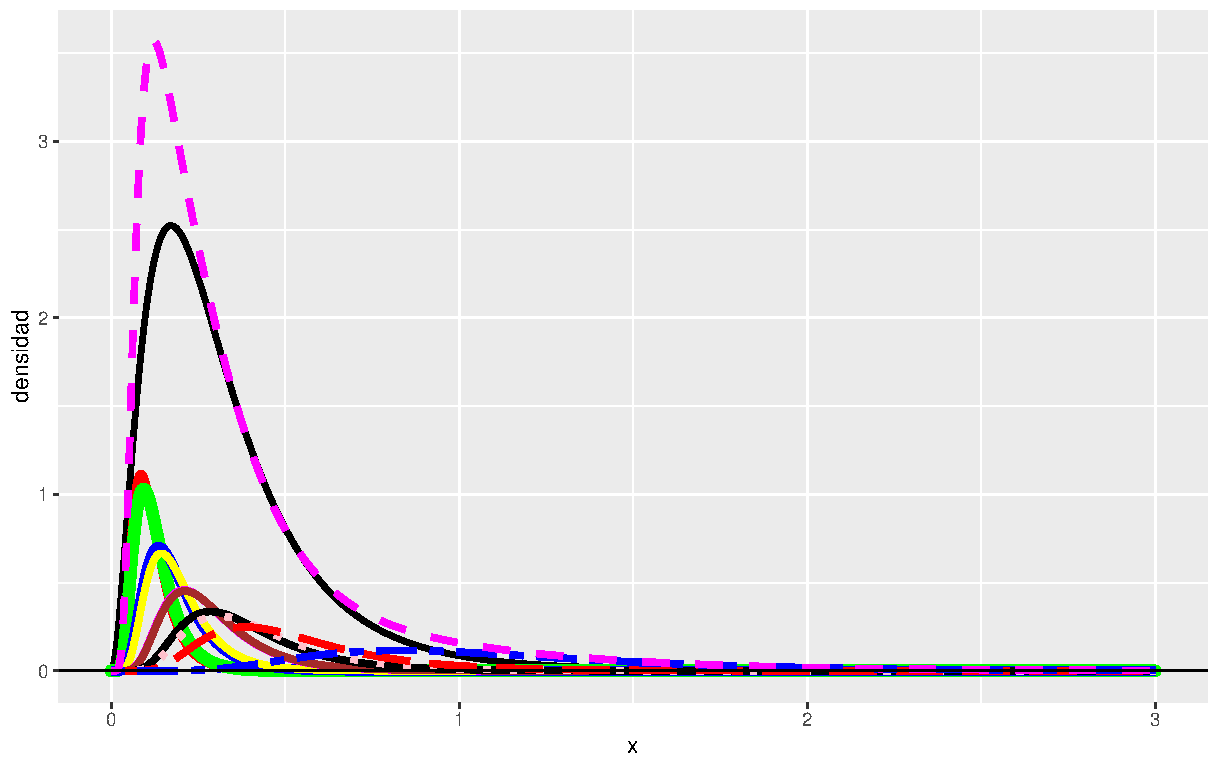
\includegraphics[scale=0.5]{../../Figures/Tesis/Capitulo5/EstimacionDensidadconLN.pdf}
	\caption{\label{EstimacionLN}Estimación de $\mathcal{G}_I^0$ para $L=3$, $\alpha=-1.5$, $\gamma=0.5$ y $n=10$}
\end{figure}

En la figura~\ref{EstimacionLN} se muestra un ejemplo de estimación de la función de densidad $\mathcal{G}_I^0$ para el caso de $\alpha=-1.5$, $\gamma=0.5$, $L=3$ y $n=10$, mediante núcleo LN donde se utilizó un ancho de banda que se obtiene de aplicar el método LSCV explicado en la subsección~\ref{AnchoBanda}. La línea sólida es la función de densidad teórica, la línea discontinua es la estimación $\widehat{f}_n$ obtenida, el resto son los distintos núcleos. Para cada $x$ el valor de $\widehat{f}_n(x)$ se obtiene como promedio de los distintos núcleos en ese $x$. Se eligió un tamaño de muestra chico para ejemplificar la metodología de estimación. Vale la pena observar que el parámetro de posición depende del valor de $x$ donde se realiza la estimación. Por eso estos núcleos cambian de forma dependiendo del valor $x$.

En la figura~\ref{EstimacionLNyGAyIG} se muestra cómo estiman los núcleos $K_{\Gamma}$, $K_{\text{\tiny{LN}}}$ y $K_{\text{\tiny{IG}}}$ al modelo $\mathcal{G}_I^0$ para un tamaño de muestra $n=25$, $L=8$ utilizando el método LSCV para elegir el ancho de banda. Se eligieron estos núcleos porque son los que finalmente evaluaremos, esta elección se justificará en el capítulo~\ref{ResultadosEmpiricos}. 
La línea solida negra es la verdadera función de densidad, se puede observar que con un tamaño de muestra no muy grande, estos núcleos ajustan bien a la función de densidad teórica.

\begin{figure}[hbt]
	\centering
	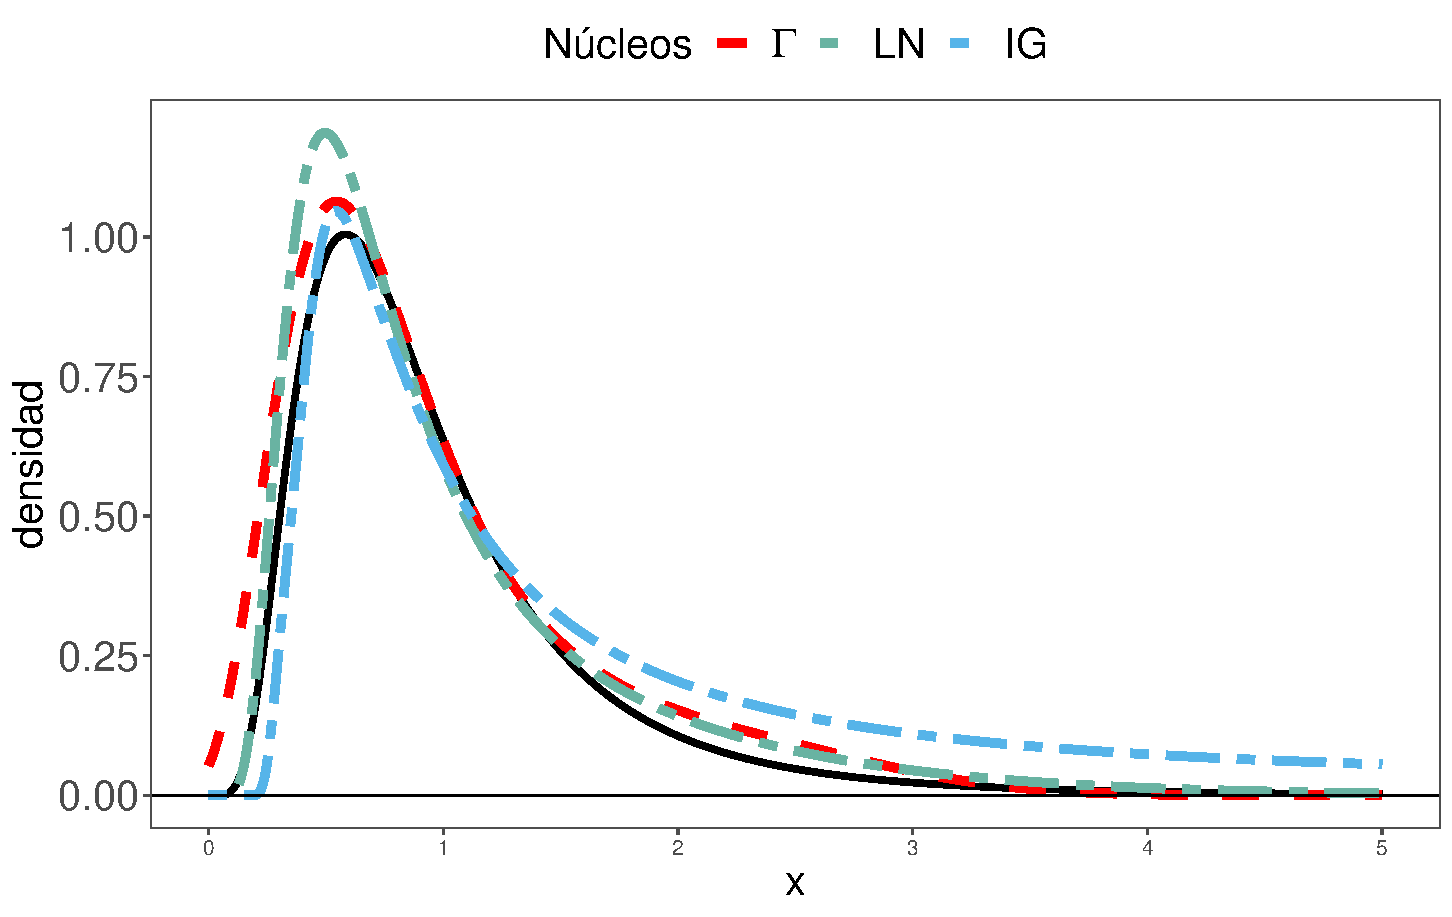
\includegraphics[scale=0.5]{../../Figures/Tesis/Capitulo5/NucleosGALNyIG.pdf}
	\caption{\label{EstimacionLNyGAyIG}Estimación de $\mathcal{G}_I^0$ para $L=8$, $\alpha=-5$, $\gamma^*=4$ y $n=25$} utilizando núcleos $K_{\Gamma}$, $K_{\text{\tiny{LN}}}$ y $K_{\text{\tiny{IG}}}$.
\end{figure}

\subsubsection{Propiedades globales}
\label{PropiedadesGlobales}

Para poder estudiar propiedades globales de estos estimadores como el MISE, se asume que:
\begin{enumerate}[a)]
	\label{CondPropGlobales}
	\item $f$ es dos veces diferenciable para todos los núcleos considerados.
	\item $\displaystyle{\int_0^{\infty}}  f'^2(x) dx$ y que $\displaystyle{\int_0^{\infty}}  (x f''(x))^2 dx$ son finitas para el caso de núcleo $\Gamma$.
	\item $\displaystyle{\int_0^{\infty}}  (x^3 f''(x))^2 dx$ es finita para el caso de los núcleos IG.
	\item $\displaystyle{\int_0^{\infty}}  \dfrac{f(x)}{x} dx$ y que $\displaystyle{\int_0^{\infty}}  (3 x f'(x)+x^2 f''(x))^2 dx$ son finitas para el caso del núcleo LN.
\end{enumerate}
Para el caso donde $f=f_{\mathcal{G}_I^0}$ las condiciones anteriores se cumplen para valores de $L$ mayores a $3/2$.

%%% ACF ¿Acá no corresponde notación matemática?
Llamaremos b* al valor del ancho de banda que minimiza el MISE, y MISE* al MISE cuando b=b*. Expresiones para b* y MISE* fueron desarrolladas por \citet{chensx2000} para el caso del núcleo $\Gamma$, y por \citet{Scaillet2004} para el caso de núcleo IG.
Se desarrollaron en el apéndice~\ref{byMiseOptLN} para el caso del núcleo LN. 

Expresiones para b* y MISE* para los núcleos $\Gamma$, IG y LN  se dan a continuación. Se considera que $b \to 0$ cuando $n \to \infty$ y $n b^a \to +\infty$ cuando $n \to +\infty$ con $a=1/2$ para los núcleos $\Gamma$, IG y $a=1$ para núcleo LN.

\begin{itemize}
	\item Núcleo $\Gamma^1$
	\begin{align}
	\label{MISEoptGamma}
	%\nonumber \text{MISE}(\widehat{f}_{\Gamma})=&b^2 \int_0^{\infty} (x f'(x)+\frac{1}{2} x f''(x))^2 dx + \frac{1}{2 \sqrt{\pi}} \frac{1}{n \sqrt{b}} \int_0^{\infty} x^{-1/2} f(x) dx \\
	%\nonumber &+ o(\frac{1}{n \sqrt{b}}+b^2)\\
	%\vspace{2cm}
	\text{b}^*_{\Gamma^1}=&\dfrac{\left[\dfrac{1}{2\sqrt{\pi}} \displaystyle{\int_{0}^{\infty}} x^{-1/2}f(x)dx \right]^{2/5}}
	{4^{2/5} \left[\displaystyle{\int_{0}^{\infty}} \left\{x f'(x) +\frac{1}{2} x f''(x)\right\}^2 dx \right]^{2/5}} n^{-2/5},\\
	\nonumber \text{MISE}^*(\widehat{f}_{\Gamma^1})=&\dfrac{5}{4^{4/5}} \left[\frac{1}{2\sqrt{\pi}} \int_{0}^{\infty} x^{-1/2}f(x)dx \right]^{4/5} \\
	&\times \left[\int_{0}^{\infty}  \left\{x f'(x) +\frac{1}{2} x f''(x)\right\}^2 dx \right]^{1/5} n^{-4/5}. 
	\end{align}
	\item Núcleo Inverso Gaussiano
	\begin{align}
	\label{MISEoptIG}
	\text{b}^*_{\text{\tiny{IG}}}=&\dfrac{\left[\dfrac{1}{2\sqrt{\pi}} \displaystyle{\int_{0}^{\infty}} x^{-3/2}f(x)dx \right]^{2/5}}
	{ \left[\int_{0}^{\infty}(x^3 f''(x))^2 dx \right]^{2/5}} n^{-2/5},\\
	\nonumber \text{MISE}^*_{\text{\tiny{IG}}}=&\dfrac{5}{4} \left[\frac{1}{2\sqrt{\pi}} \displaystyle{\int_{0}^{\infty}} x^{-3/2}f(x)dx \right]^{4/5} \\
	&\times \left[\displaystyle{\int_{0}^{\infty}}  \left\{x^3 f''(x) \right\}^2 dx \right]^{1/5} n^{-4/5} .
	\end{align}
	\item Núcleo Lognormal
	\begin{align}
	\label{MISEoptLN}
	\text{b}^*_{\text{\tiny{LN}}}=&\dfrac{\left[\dfrac{1}{2\sqrt{\pi}}\displaystyle{\int_0^{+\infty}}\frac{f(x)}{x}\right]^{1/5}}{\left[\displaystyle{\int_0^{+\infty}} x^2(3f'(x)+xf''(x))^2\right]^{1/5}}n^{-1/5},\\
	\nonumber \text{MISE}^*_{\text{\tiny{LN}}}=&\dfrac{5}{4}  \left[\dfrac{1}{2\sqrt{\pi}}\displaystyle{\int_{0}^{\infty}} \frac{f(x)}{x} \right]^{4/5} \\
	&\times \left[\displaystyle{\int_{0}^{\infty}}  x^2 (3 f'(x) + x f''(x))^2 \right]^{1/5} n^{-4/5}.
	\end{align}
\end{itemize}

Por lo tanto, $\widehat{f}_{\Gamma^1}$, $\widehat{f}_{\tiny{\text{IG}}}$ y $\widehat{f}_{\tiny{\text{LN}}}$ alcanzan una tasa de convergencia en términos del MISE del orden de $n^{-4/5}$, comparable con la que alcanzan otros núcleos simétricos.

%%In \citet{bouezmarni2005} the authors prove, among others results, that under certain conditions for the bandwidth, $\widehat{f}_n$ converges to $f$  in probability, in $L_1$ sense.
%In \citet{bouezmarni2005} the authors prove several theoretical results for this estimator. 
%One of them is that, under certain conditions for the bandwidth, $\widehat{f}_n$ converges to $f$  in probability, in $L_1$ sense.

\subsection{Ancho de banda}
\label{AnchoBanda}

La elección del ancho de banda $b$ es un punto crucial en estimación no paramétrica de la función de densidad. Si $b$ es muy pequeño la función de densidad estimada puede ser muy ruidosa. Si en cambio, el valor de $b$ es demasiado grande, entonces la estimación puede pasar por alto características clave porque la variabilidad disminuye.

En esta tesis se estudiarán dos estrategias para determinar el ancho de banda $b$.

\begin{itemize}
	%\item El $b_{opt}$ que es el valor de $b$ que minimiza el MISE. Expresiones de $b_{opt}$ se darán en la siguiente subsección.
	\item Un valor específico de $b$ encontrado empíricamente.
	\item El método Least Squared Cross Validation (LSCV) ampliamente utilizado en la literatura.
\end{itemize}


El método LSCV consiste en encontrar el valor de $b$ que minimiza una aproximación del ISE. Observemos que, dada una muestra,
\begin{align}
\label{ISE}
\text{ISE}(b)=&\int_\mathbb{R} (\widehat{f}_b-f)^2 dx \nonumber\\ 
=& \int_\mathbb{R} \widehat{f}_b^2dx- 2 \int_\mathbb{R} \widehat{f}_b fdx +\int_\mathbb{R} f^2dx.
\end{align}

El último término de la ecuación~\eqref{ISE} no depende de $b$. Entonces
\begin{align}
\nonumber \min_b \text{ISE}(b)= \min_b \phi(\widehat{f}_b) \text{ donde } ,
\end{align}
donde
\begin{align}
\label{fi}
\phi(\widehat{f})=\int_\mathbb{R} \widehat{f}_b^2 dx- 2 \int_\mathbb{R} \widehat{f}_b fdx.
\end{align}

Notemos que el segundo término de la ecuación~\eqref{fi} se puede ver como $E_\text{X}(\widehat{f}_b(x))$ con $X \sim f$ desconocida. Por lo tanto se puede estimar $E_\text{X}(\widehat{f}_b(x)$ por medio de $\widehat{E}_\text{X}(\widehat{f}(x))=\frac{1}{n}\sum_{i=1}^n \widehat{f}(X_i)$. 
Notemos que la observación $X_i$ donde se evalúa $\widehat{f}$ es utilizada también para encontrar $\widehat{f}_b$. Una forma de asegurar independencia entre $X_i$ y  $\widehat{f}_b$ es considerar el \textit{leave-one out} estimador:
\begin{align}
\widehat{E}_\text{X}(\widehat{f}_b(x))=\frac{1}{n}\sum_{i=1}^n \widehat{f}_{b,-i}(X_i),
\end{align}	
que es el estimador de $\widehat{f}_{b,-i}$ sin considerar la $i$-ésima observación. 
De esta forma nos aseguramos que las observaciones utilizadas para calcular  $\widehat{f}(\cdot)$ son independientes de $X_i.$
%$\widehat{f}_{-i}(x)= \widehat{f}_{i;h}(x)=\dfrac{1}{n} \displaystyle{\sum_{j=1,j\neq i}^n} K_{(x,h)}(X_i)$

El valor de $b_{\tiny \text{LSCV}}$ óptimo que propone este método es aquel valor que minimiza la función de validación cruzada
\begin{align}
\label{LSCV}
\text{LSCV}(b)=\int_\mathbb{R} \widehat{f}_b^2(x)dx - \frac{2}{n}\sum_{i=1}^n \widehat{f}_{b,-i}(X_i).
\end{align}
 \citet{HallMarron1991} muestran que, para el caso de núcleos simétricos, esta función puede tener mínimos locales. Entonces el  $b_{\tiny \text{LSCV}}$ será el más grande de los mínimos locales porque tiene un mejor comportamiento empírico que el mínimo global.

En la figura~\ref{LSCVgraf} se puede ver la función de validación cruzada LSCV en función del ancho de banda, usando núcleo $\Gamma$, para $L=3$, $\alpha=\{-3,-5\}$ y $n=\{9,25,49,81,121\}$. Se puede ver que, en todos los casos, esta función presenta un único mínimo.

\begin{figure}[hbt]
	\centering 
	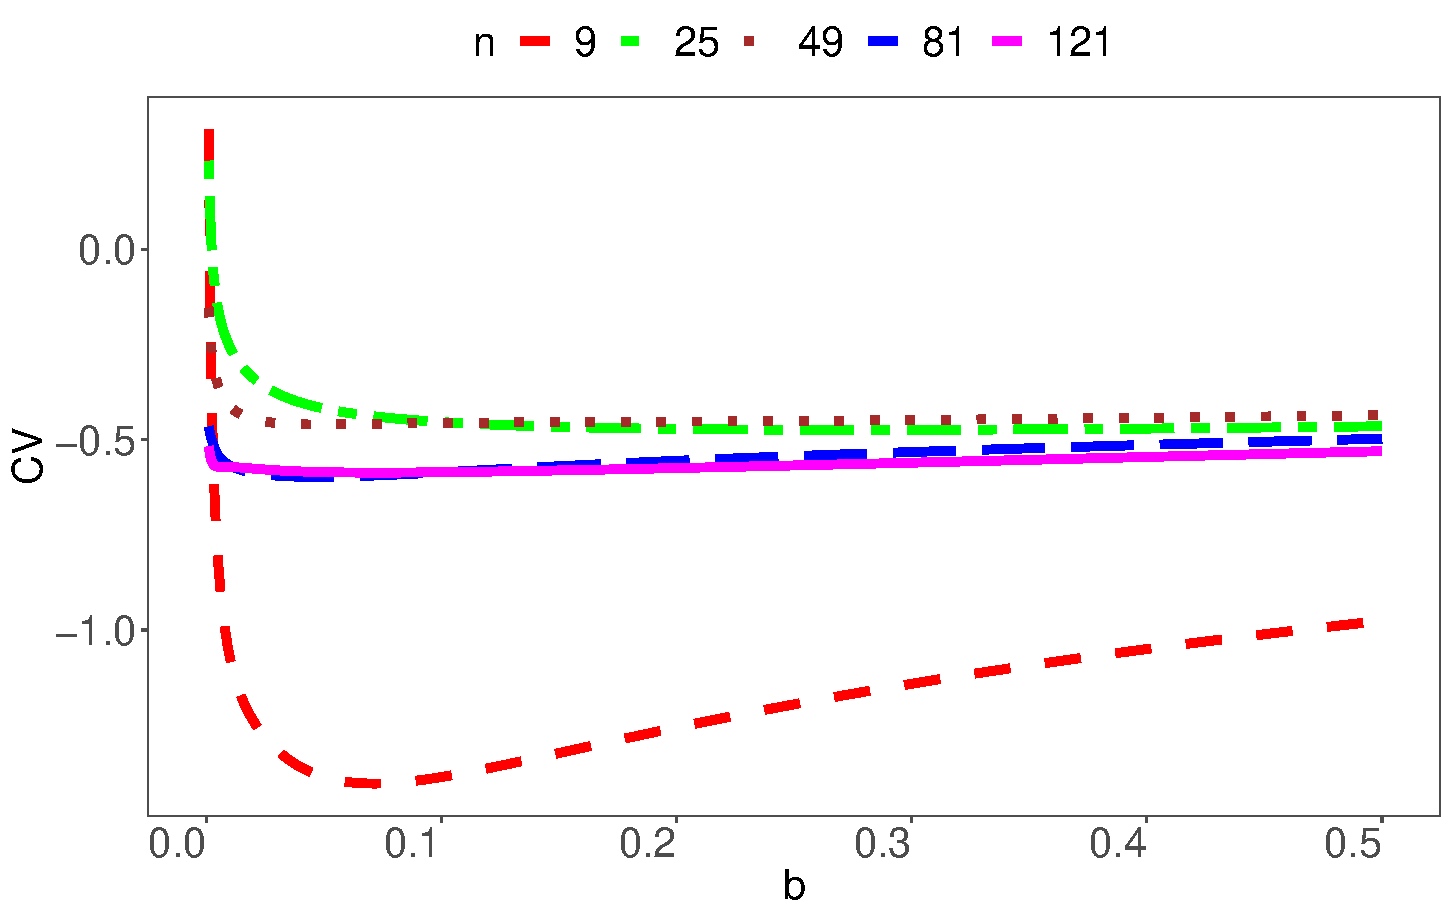
\includegraphics[scale=0.5]{../../Figures/Tesis/Capitulo5/GraficoLSCValfa=-5.pdf}
	\caption{\label{LSCVgraf} Least Square Cross Validation (LSCV) para $L=3$ y $\alpha=-5$}
\end{figure}

%\begin{figure}[hbt]
%	\centering    
%	\label{MV}
%	\subfigure[$\alpha=-1.5$]{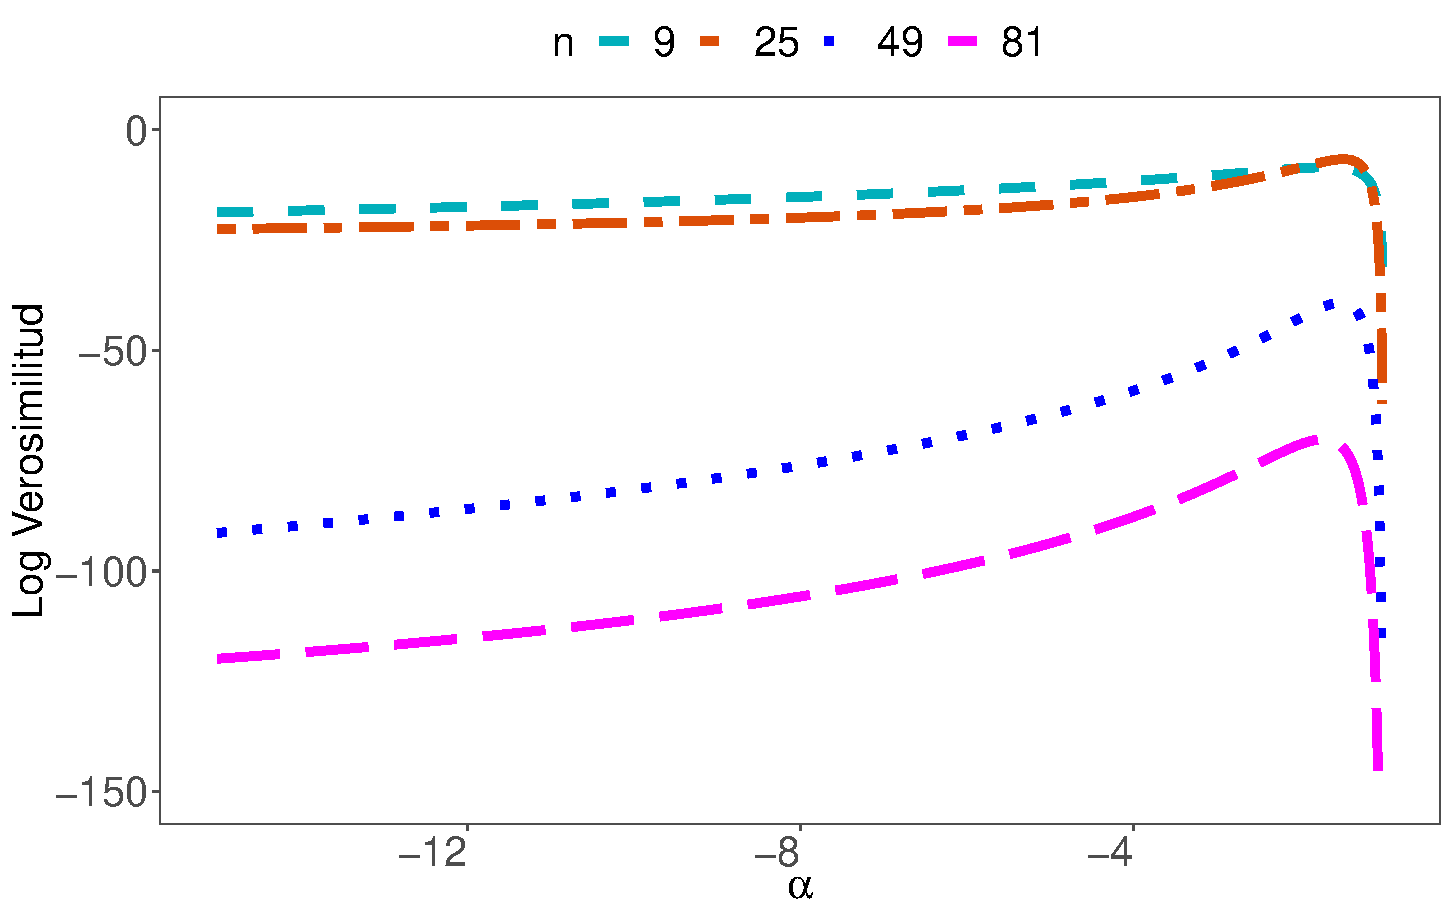
\includegraphics[scale=0.5]{../../Figures/Tesis/Capitulo5/Verosimilitud1punto5_2.pdf}}
%	\subfigure[$\alpha=-5$]{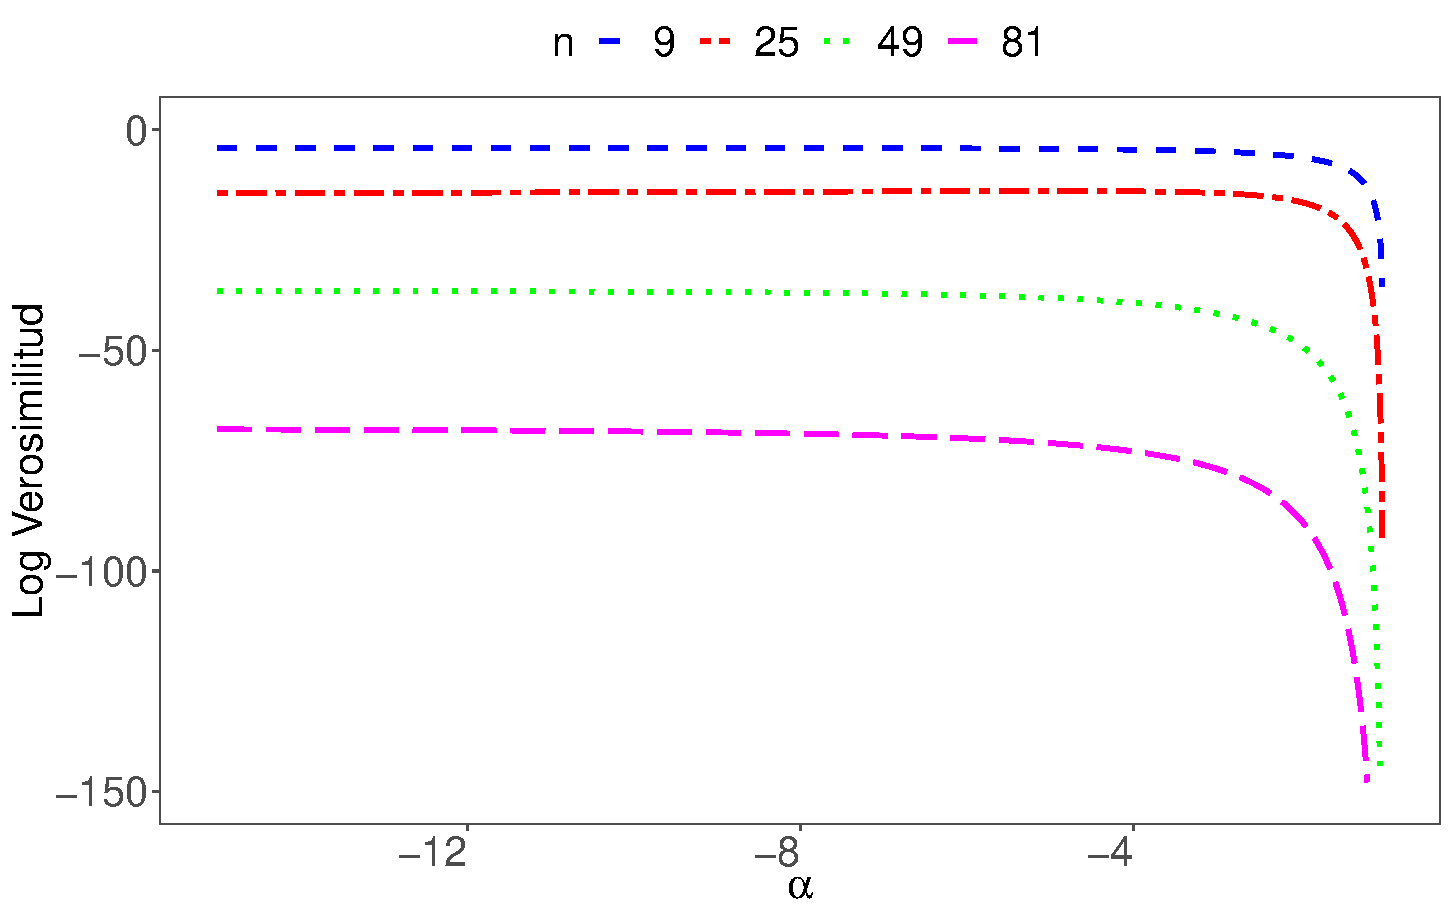
\includegraphics[scale=0.5]{../../Figures/Tesis/Capitulo5/Verosimilitud-5_2.pdf}}
%	\caption{Función de verosimilitud para $L=3$}
%\end{figure}

%\item It is possible to see that (\ref{LSCV}) in an unbiased estimator of (\ref{fi}).
%\item In 1991, Hall and Marron  \citet{HallMarron1991},  pointed out that the function (\ref*{LSCV}) has frequent local minima. For this reason, the largest local minimizer (which gives better empirical
%performance than the global minimizer) is the $b_{LSCV}$.
%SE PUEDE VER QUE \ref(LSCV) es un estimador insesgado de \ref{fi}

%\end{frame}		


\subsubsection{Convergencia}

Es interesante contar con resultados de convergencia de un estimador para medir la calidad del mismo. \citet{Libnegue2013} presenta propiedades asintóticas del estimador $\widehat{f}_n$ de $f$, donde $\widehat{f}_n$ es el estimador de núcleos asimétricos dado en la definición~\ref{DefNucleo}. De acuerdo a los trabajos de \citet{Libnegue2013,kokonendji2018} se consideran los núcleos que verifican las condiciones: 
\begin{align}
\label{CondNucleos}
\begin{split}
x \in \text{Soporte}(K_{x,b}),\\
E(Y_{x,b})=x+A(x,b),\\
Var(Y_{x,b})=B(x,b),
\end{split}
\end{align}
donde $Y_{x,b}$ es una variable aleatoria con densidad $K_{x,b}$ y $A(x,b),B(x,b) \to 0$ cuando $b \to 0$. Tanto el núcleo $\Gamma^1$ como los núcleos LN e IG verifican estas condiciones, pues:
\begin{itemize}
	\item para el núcleo $\Gamma^1$, $A(x,b)=b$ y $B(X,b)=b(x+b)$.
	\item para el núcleo LN, $A(x,b)=x(e^{\frac{3}{2} b^2}-1)$ y $B(X,b)=x^2 e^{3b^2} (e^{b^2}-1)$.
	\item para el núcleo IG, $A(x,b)=0$ y $B(X,b)=x^3 b$.
\end{itemize}

En estos mismos trabajos se demuestran resultados de consistencia y de normalidad asintótica, como así también se demuestran propiedades de convergencia globales. Algunos de estos resultados son necesarios para probar la consistencia del estimador del parámetro de textura de la distribución $\mathcal{G}_I^0$ que se propone en esta tesis y que presentaremos en la sección~\ref{MDE}.

%En este capítulo, presentamos un estudio general de las propiedades asintóticas.
%en la familia de los estimadores de núcleo asociados continuos bfn o efn, que dependen intrínsecamente de
%punto de estimación x y parámetro de suavizado h, para funciones
%de densidad de soporte T = TI limitada al menos en un lado. Para enfatizar la sensibilidad
%diferentes puntos de la estimación (en los bordes y en el interior), proponemos
%utilizar técnicas simples, que logran los mismos resultados pero con
%más flexible que en el caso clásico y que depende en gran medida de
%situación del punto de estimación xy una cierta potencia del parámetro de suavizado
%h. La suposición de la continuidad uniforme de f en T = R se relaja en una continuidad simple
%de f en cualquier TI compacta. 
%
%Sea f ∈ C2 (TI) la densidad a estimar y bfn su estimador de núcleo asociado
%definido en (3.1). Para cada punto x fijo en T, tenemos
%
%Consistencia débil uniforme en cada conjunto compacto en
%[0; +1) se prueba para estos estimadores cuando f es continua en su soporte.
%También se establece una convergencia débil en $\text{L}_1$. Finalmente probamos
%que el estimador asimétrico de densidad del núcleo y el histograma suavizado
%convergen en probabilidad a infinito en x = 0 cuando la densidad
%no tiene límites en x = 0.

%En esta sección daremos algunos resulados de convergencia de los núcleos presentados que fueron demostrados en Bouezmarni et al. \citet{bouezmarni2005} y en XXXXXXXX para los núcleos asimétricos \text{A}_n, donde $\text{A}_n$ son los núcleos $K_{\Gamma}$, $K_{\tiny \text{IG}}$ y $K_{\tiny \text{RIG}}$. 
\begin{itemize}
	\item \textbf{Convergencia fuerte de $\widehat{f}_n$} 

	\begin{theorem}
		\label{ConvFuerte_fn}
		Sea $f \in C^2(\text{Soporte}(f))$ la densidad a estimar, donde $\text{Soporte}(f)$ es el soporte de $f$, y $\widehat{f}_n$ el estimador  de $f$ por núcleos dado en la definición~\ref{DefNucleo} y que verifican las condiciones~\ref{CondNucleos}. Para cualquier punto $x$ fijo en $\text{Soporte}(f)$ tenemos que si $b \to +\infty$ cuando $n \to +\infty$ entonces
		\begin{align}
		\widehat{f}_n(x) \xrightarrow{\;\; c.s. \;\; }f(x) \; \text{ cuando } \; n \rightarrow \infty.
		\label{Consistenciac.s.} 
		\end{align}	
%		Además, si existe un número real $r_2=r_2(K_x,b_n)>0$ tal que 
%		\begin{align}
%		b_n^{r_2}\left\lVert K_{x,b_n}\right\rVert_2^2 \leq c_2(x)<+\infty \text{ y } \lim\limits_{n \rightarrow \infty} n \, b_n^{2a}=+\infty \text{ entonces}\\
%		\centering \widehat{f}_n(x) \xrightarrow{\;\; \mathbb{L}^2 \;\; }f(x) \; \text{ cuando } \; n \rightarrow \infty.
%		\label{ConsistenciaL2} 
%		\end{align}	
\end{theorem}
%\end{itemize}

%Cabe señalar que el valor de $r_2=\frac{1}{2}$ para los núcleos $K_{\Gamma}$ y $K_{\tiny \text{IG}}$, mientras que $r_2=1$ para el núcleo $K_{\tiny \text{LN}}$.

%\begin{itemize}
%	\item \textbf{Convergencia uniforme del sesgo.} 
%	\begin{theorem}
%		Sea $f$ una función de densidad continua y acotada en su soporte, $\widehat{f}_{\tiny \text{A}_n}$ el estimador de $f$ utilizando núcleos definidos en \citet{Libnegue2013} dentro de los cuales se encuentran $K_{\Gamma}$, $K_{\tiny \text{IG}}$ y $K_{\tiny \text{LN}}$. Para todo conjunto compacto $I \subset \text{Soporte}(f)$ se cumple que
%		\begin{align}
%			\sup_{x \in I} |\mathbb{E}(\widehat{f}_n(x))-f(x)|\xrightarrow{\;\;  \;\; }0 \; \text{ cuando } \; n \rightarrow \infty.
%			\label{convergenciaProb} 
%		\end{align}
%	\end{theorem}


%\begin{itemize}
%	\item \textbf{Convergencia débil y fuerte de $\widehat{f}_n$.} 
%\begin{theorem}
%	Sea $f$ una función de densidad continua y acotada en en su soporte, $\widehat{f}_{\tiny \text{A}_n}$ el estimador de $f$ utilizando núcleos definidos en \citet{Libnegue2013} dentro de los cuales se encuentran $K_{\Gamma}$, $K_{\tiny \text{IG}}$ y $K_{\tiny \text{LN}}$. Sea $I$ un conjunto compacto en $\text{Soporte}(f)$. Entonces si existe un número real $r_0=r_0(K)>0$ que depende del núcleo elegido, tal que para todo $x \in \text{Soporte}(f)$ 
%	\begin{align}
%	b_n^{r_0} \displaystyle{\int_0^{\infty}} | dK_{x,b_n}(s) | \leq c_0(x),
%	\end{align}
%	donde $c_0(x)$ es una función acotada superiormente en cualquier compacto que contenga a $x$. Entonces, para todo subconjunto compacto $I \subset \text{Soporte}(f)$ con $\lim\limits_{n \rightarrow \infty} b_n=0 $ tenemos que:
%	\begin{enumerate}[a)]
%		\item $\lim\limits_{n \rightarrow \infty} n \, b_n^{2a}=+\infty$,  entonces
%		\begin{align}
%		\sup_{x \in I} |\widehat{f}_n(x)-f(x)|\xrightarrow{\;\; \Pr \;\; }0 \; \text{ cuando } \; n \rightarrow \infty.
%		\label{convergenciaProb} 
%		\end{align}
%		\item $\lim\limits_{n \to \infty} \dfrac{n b_n^{2a}}{\ln{n}}  = +\infty $, entonces 
%		\begin{align}
%		\sup_{x \in I} |\widehat{f}_n(x)-f(x)|\xrightarrow{\;\; c.s. \;\; }0 \; as \; n \rightarrow \infty ,
%		\label{convergencia.a.s.}
%		\end{align}
%	\end{enumerate}
%con $r_0=1$ para el núcleo $K_{\Gamma}$, $r_0=5/2$ para $K_{\tiny \text{IG}}$, y $r_0=2$ para el núcleo $K_{\tiny \text{LN}}$. 
%\end{theorem}

Si se considera un conjunto de condiciones más fuertes sobre el ancho de banda se obtienen resultados sobre la convergencia en $L_1$. 

%\begin{itemize}
%	\item Consistencia fuerte uniforme de $\widehat{f}_n$.
%\begin{corollary}
%	Sea $f$ una función de densidad definida en $[0;+\infty)$ y $\widehat{f}_n$ el estimador de la densidad $f$ utilizando núcleos asimétricos. Entonces, si $\lim\limits_{n \to \infty} b = 0 \text{ and} \lim\limits_{n \to \infty} \dfrac{n b^{2a}}{\ln{n}}  = +\infty $,
%	\begin{equation}
%	\sup_{x \in I} |\widehat{f}_n(x)-f(x)|\xrightarrow{\;\; a.s. \;\; }0 \; as \; n \rightarrow \infty 
%	\label{a.s.}
%	\end{equation}
%	con $a = 1$ el núcleo $\Gamma$ and $a = \frac{5}{2}$ para los núcleos IG y RIG respectivamente.
%\end{corollary}
%\end{itemize}


\item \textbf{Convergencia en $\text{L}_1$ de $\widehat{f}_n$}

\begin{theorem}
	\label{ConvergenciaFuerte}
	\bigskip
	Sea $f$ una función de densidad continua y acotada en $\text{Soporte}(f)$.
	Sea $\widehat{f}_{n}$ el estimador de $f$ utilizando núcleos definidos en~\ref{DefNucleo} y que verifica las condiciones~\ref{CondNucleos}. Supongamos que existe un número real $r_1=r_1(K)>0$ que depende del núcleo elegido tal que, para cada $x \in \text{Soporte}(f)$ 
	\begin{align}
	\label{cond_c1}
	b_n^{r_1} \displaystyle{\int_0^{\infty}} | dK_{x,b_n}(s) | \leq c_1(x),
	\end{align}
	donde $c_1(x)$ es una función integrable en cualquier compacto que contenga a $x \in \text{Soporte}(f)$. Entonces si $\lim\limits_{n \rightarrow \infty} b_n=0 $ y
	\begin{enumerate}[a)]
		\item $\lim\limits_{n \rightarrow \infty} n \, b_n^{2r_1}=+\infty$,  entonces
		\begin{align}
		\int_0^{+\infty} \vert \widehat{f}_n(x)-f(x)\vert dx \stackrel{p} {\longrightarrow} 0 \text{ cuando } n \rightarrow \infty.
		\label{L1debil}
		\end{align}
		\item $\lim\limits_{n \to \infty} \dfrac{n b^{2r_1}}{\ln{n}}  = +\infty $, entonces 
		\begin{align}
		\int_0^{+\infty} \vert \widehat{f}_n(x)-f(x)\vert dx \stackrel{c.s.} {\longrightarrow} 0 \text{ cuando } n \rightarrow \infty.
		\label{L1fuerte}
		\end{align}
	\end{enumerate}
\end{theorem}

\end{itemize}

\citet{Libnegue2013} muestra que la condición~\ref{cond_c1} se cumple para $r_1=1$ en el caso del núcleo $\Gamma^1$, $r_1=2$ para el núcleo LN y $r_1=5/2$ para el núcleo IG.

El resultado~\ref{L1fuerte} es esencial para demostrar la consistencia fuerte del estimador de mínima distancia para el parámetro de textura $\alpha$ de la distribución $\mathcal{G}_I^0$ como veremos en sección~\ref{MDE}.

%Choosing Bandwidths in Practice
%Picking the best smoothing parameter from data is an important task in
%practice. If the smoothing parameter is too small, the estimate is too noisy,
%exhibiting high various and extraneous wiggles. If the smoothing parameter
%is too large, then the estimate may miss key features due to oversmoothing,
%washing out small details. Such estimates have low variance but high bias in
%many regions. In practice, bandwidths that do not differ by more than 10-15%
%from the optimal bandwidth are usually satisfactory.
%
%	\begin{itemize}
%	\item All the asymmetric kernel estimator studied are free of boundary bias, always non-negative and have an optimal rate of convergence of $n^{-\frac{4}{5}}$ for the mean integrated squared error.
%	\medskip	
%	\item Assuming that $f$ has continuous second derivative and:
%	\begin{itemize}
%		\item $\int_0^{\infty} f'^2(x)dx \text{ and } \int_0^{\infty} (xf''(x))^2dx$ are finite for Gamma kernel estimator.
%		\medskip
%		\item $\int_0^{\infty} (x^3f''(x))^2dx$ is finite for IG and RIG kernel estimator.
%		\medskip
%		\item $\int_0^{\infty} x f'(x)dx \text{ and }\int_0^{\infty} (x^2f''(x))^2dx$ is finite for $LN$ kernel estimator.
%		\medskip
%	\end{itemize}
%	expression of optimal bandwidth $b$, one that mimimizes MISE, can be obtained.
%	\medskip
%	%	\item These expressions depends on these integrals.
%\end{itemize}
%
%
%
%
%	\begin{itemize}
%		\item Uniform Strong Consistency of $\widehat{f}_b$.\\
%		\bigskip
%		Let $f$ be a continuous and bounded probability density function on $[0, \infty)$, $\widehat{f}_b$, the asymmetric kernel density estimator, and $I$ a compact set in $[0, \infty)$. 
%		Under the two conditions:
%		$$b \rightarrow 0 \ \ \text {and} \ \  \frac{n \, b^{2a}}{\ln(n)} \rightarrow +\infty$$
%		we have
%		\begin{align*}
%		\sup_{x \in I} |\widehat{f}_b(x)-f(x)|\xrightarrow{\;\; a.s. \;\; }0 \; as \; n \rightarrow \infty 
%		\end{align*}
%		where $a=1$ for the gamma kernel and $a=5/2$ for the inverse Gaussian and reciprocal inverse Gaussian kernels.
%	\end{itemize}
%
%Estimation of unbounded densities at $x=0$
%	\begin{itemize}
%		\item Sufficient conditions needed to get weak convergence of the asymmetric kernel density estimator to infinity at $x=0$.\\
%		\medskip
%		Let $f$ be a probability density function on $[0, \infty)$, unbounded at $x=0$. Under the condition 
%		$$\lim_{n \rightarrow \infty} b=0 \  \text{and} \ \lim_{n \rightarrow \infty} n \, b^{2a}=+\infty \, (a>0)$$
%		we have
%		$$\widehat{f}_b \xrightarrow{\;\; \Pr \;\; } +\infty \  \  as \  \  n \rightarrow \infty$$
%		if 
%		$$\forall \delta > 0, \, \int_0^\delta K(0,b)(t)dt \rightarrow 1 \ \ as \ \ b \rightarrow 0$$
%		\item It shows thay the asymmetric kernel estimator gives almost all weight to the boundary point when de bandwidth converges to zero.
%	\end{itemize}

%%%%%%%%%%%%%%%%% VEEERRR si lo pongo
%VER ABAJO COMENTADO


%\item Explicit expression of $b_{opt}$ can be obtained for $L\geq \dfrac{3}{2}$.
%\medskip
%\item Because the integrals converge for $L\geq \dfrac{3}{2}$.
%\medskip
%\item $L=1$ case is studied with Extrem Theory Values.

\subsection{Distancias Estocásticas}

Al momento de proponer un modelo estadístico es importante contar con una medida apropiada que indique la diferencia entre el modelo teórico y los datos muestrales. Si nos basamos en la información muestral existen medidas que vinculan la función de distribución empírica y el modelo teórico, y otras que miden la discrepancia entre una estimación no paramétrica de la función de densidad subyacente y la función de densidad que proviene del modelo utilizado. En esta tesis se trabajará con esta última propuesta.

Es conocido el aporte que realizó Claude E.\ Shannon a la creaci\'on de lo que se conoce como \textit{Teoría de la Información}. \citet{Shannon1948} propone una nueva manera de medir la transmisi\'on de informaci\'on a trav\'es de un canal, pensando a la informaci\'on como un concepto estad\'istico. Propone como medida de informaci\'on o de desorden a lo que se conoce como entrop\'ia de Shannon. En el caso discreto y considerando $X$ una variable aleatoria que toma $n$ valores con probabilidades $p_1,\ldots,p_n$, entonces la entrop\'ia de Shannon se define como $H(X)=-\sum_{i=1}^n p_i \log p_i$. Para el caso continuo se define $H(X)=-\int_{-\infty}^{\infty} f_X(x) \log f_X(x)$ donde $f$ es la función de densidad de probabilidad de la variable aleatoria $X$.

 \citet{KullbackLeibler1951} (KL) estaban interesados en proponer una medida que discrimine dos poblaciones, considerando una cantidad que involucre medidas de informaci\'on. Su inter\'es era definir una magnitud que indique la diferencia entre dos funciones de distribuci\'on pensando en una generalizaci\'on de la entrop\'ia de Shannon. Si $p(x)$ y $q(x)$ son dos funciones de probabilidad puntual con el mismo soporte $\Omega$, la KL divergencia se define como $d_{\text{\tiny{KL}}}(p \rVert q)=-\sum_{x \in \Omega} p(x) \log \dfrac{q(x)}{p(x)}=\sum_{x \in \Omega} p(x) \log\dfrac{p(x)}{q(x)}$. 

En el caso continuo la divergencia KL se define como 
\begin{align}
\label{KL}
d_{\text{\tiny{KL}}}(f \rVert g)=\int_{-\infty}^{+\infty} f(x) \log\dfrac{f(x)}{g(x)} dx,
\end{align} 
donde $f(x)$ y $g(x)$ representan funciones de densidad. 

Se puede pensar que si $f$ es el modelo verdadero, la KL divergencia mide cu\'anto me alejo del modelo verdadero, si utilizo el modelo $g$ en vez del modelo $f$. Hay que notar que si $f=g$ la distancia $d_\text{\tiny{KL}}=0.$ Esta medida de ``distancia'' no es sim\'etrica ni cumple con la desigualdad triangular,  en cambio s\'i cumple que $d_{\text{\tiny{KL}}}(f \rVert g)\geq 0$ y $d_{\text{\tiny{KL}}}(f \rVert g)= 0 \Longleftrightarrow f=g.$ 

Muchas de las medidas utilizadas que se basan en determinar diferencias entre una estimación de la función de densidad subyacente y el modelo teórico no son métricas, donde por métrica entendemos a aquellas funciones $D:M \times M\rightarrow \mathbb{R}^+$ que cumplen:

\begin{enumerate}
	\label{metrica}
	\item \label{positiva}$D(x,y)\geq 0$ $\forall x,y \in M$.
	\item \label{igual0}$D(x,y)= 0 \Leftrightarrow x=y$.
	\item \label{simetrica}$D(x,y)=D(y,x)$  $\forall x,y \in M$.
	\item \label{DesigTriang}$D(x,z)\leq D(x,y)+D(y,z)$  $\forall x,y,z \in M$.
\end{enumerate} 

Es decir, son medidas que no cumplen la propiedad~\ref{simetrica} ni~\ref{DesigTriang}, pero sí cumplen las propiedades~\ref{positiva} y~\ref{igual0}. 
Si la medida de discrepancia cumple solamente las propiedades~\ref{positiva} y~\ref{igual0} la llamaremos ``divergencia''. 
Si además cumple la propiedad~\ref{simetrica} de simetría, la llamaremos ``distancia estocástica''. 

\citet{Salicru1994} propusieron una familia de medidas de divergencia, llamadas $(h,\phi)$-divergencias que incluyen a la KL divergencia, a las $\phi$-divergencias presentadas por \citet{Csiszar1967} y a las generalizaciones de las $J$- divergencias y $R$-divergencias que fueron definidas por \citet{Taneja1989} entre otras. Algunas de las medidas que se trabajan en esta tesis son $\phi$ divergencias y otras  $(h,\phi)$- divergencias. 
Por eso daremos la definición de ambas.

En el análisis de imágenes SAR, \citet{Nascimento2009} estudiaron estas medidas en el contexto de abordar el problema de cuantificar cuán distinguibles son dos regiones de una imagen entre sí.

\begin{definition}[$\phi$-divergencias]
	\label{fiDivergencia}
	Sean $F(x)$ y $G(x)$ dos funciones de distribución definidas sobre el mismo conjunto $S \subset \mathbb{R}$, ambas absolutamente continuas con respecto a la medida Lebesgue, es decir existen $f(x)$ y $g(x)$ funciones de densidad correspondientes a $F$ y $G$ respectivamente. Además $F(x)$ absolutamente continua con respecto a $G(x)$, entonces para toda función convexa $\phi:[0,+\infty)\rightarrow \mathbb{R}$ tal que $\phi(1)=0$, la $\phi$-divergencia entre $f$ y $g$ se define como
	\begin{align}
	d_{\phi}(f, g)=\int_{S}  \phi\left(\dfrac{f(x)}{g(x)}\right) g(x) dx=E_{g}\left(\phi\left(\dfrac{f}{g}\right)\right).
	\end{align}
	%donde $f_{\theta_1}$ y $f_{\theta_2}$ las funciones de densidad de $F_{\theta_1}$ y $F_{\theta_2}$ respectivamente.
\end{definition}

Cabe realizar algunas observaciones:

\begin{itemize}
	\item Por la desigualdad de Jensen y por ser $f$ una función de densidad se verifica que:
	\begin{align}
	\displaystyle \int_{S} \phi\left(\dfrac{f(x)}{g(x)}\right) g(x) dx \geq \phi\left(\int_{S} \dfrac{f(x)}{g(x)} g(x) dx\right)=\phi(1)\cdot
	\end{align}
	Entonces, la condición $\phi(1)=0$ garantiza que la medida de divergencia cumpla que $d_{\phi}(f, g) \geq 0.$ Además, si $f=g$ entonces $d_{\phi}(f, f)= 0.$ 
	\item La condición que $F(x)$ sea absolutamente continua con respecto a $G(x)$ es equivalente a pedir que, en casi todo punto, $\text{Soporte}(g) \subset \text{Soporte}(f).$ En general, en la literatura se pide que ambas funciones de densidad tengan un soporte común.
\end{itemize}

\begin{example} Ejemplos de $\phi$-divergencias. En estos ejemplos asumiremos que $f$ y $g$ tienen soporte común $S$.
	\begin{itemize}
		\item Kullback-Leibler definida en~\eqref{KL} donde $\phi(x)=x \log(x)$.
		\item Hellinger
		\begin{align} 
		d_{\text{\tiny{H}}}(f,g)=\dfrac{1}{2} \displaystyle \int_{S} \left(\sqrt{f(x)}-\sqrt{g(x)}\right)^2 dx,
		\end{align}
		donde $\phi(x)=\left(\sqrt{x}-1\right)^2$.
		\item Triangular
		\begin{align}
		\label{triangular}
		d_{\text{\tiny{T}}}(f,g)=\displaystyle \int_{S} \dfrac{\left(f(x)-g(x)\right)^2}{f(x)+g(x)} \ dx,
		\end{align}
		donde $\phi(x)=\dfrac{\left(x-1 \right)^2}{x+1}$.
	\end{itemize}
\end{example}

\begin{definition} $(h,\phi)$-divergencias.
	\label{hfiDivergencia}
	Si se mantienen las hipótesis dadas en la definición~(\ref{fiDivergencia}) y $h: (0,+\infty)\rightarrow [0,+\infty)$ es una función estrictamente creciente que verifica que $h(0)=0$ entonces se define la $(h,\phi)$-divergencia como
	\begin{align}
	d^h_{\phi}(f, g)=h\left(\int_{S} \phi\left(\dfrac{f(x)}{g(x)}\right) g(x) \ dx\right)=h\left(E_{g}\left(\phi\left(\dfrac{f}{g}\right)\right)\right).
	\end{align}
\end{definition}
%	Distancia de Bhattacharyya $d_B(V,W)=-\log\int_{-\infty}^{\infty}\sqrt{f_Vf_W}$.
%	\item Distancia Triangular $d_T(V,W)=\int_{-\infty}^{\infty}\frac{(f_V-f_W)^2}{f_V+f_W}$.
%	\item Distancia de R\'enyi con parámetro $\beta\in(0,1)$

\begin{example} Ejemplos de $(h,\phi)$-divergencia son:
	\begin{itemize}
		\item Bhattacharyya 
		\begin{align}
		\label{Bhattacharyya}
		d_{\text{\tiny{B}}}(f,g)=-\log \displaystyle \int_{S} \sqrt{f(x) g(x)} dx,
		\end{align}
		donde $\phi(x)=-\sqrt{x}+\dfrac{x+1}{2}$ y $h(y)=-\log(-y+1)$ con $0\leq y<1$.
		\item R\'enyi de orden $\beta\in(0,1)$ simetrizada.
		\begin{align}
		d_\text{\tiny{R}}^{\beta}(f,g)=\frac{1}{2(\beta-1)}\left[\log\int_{S}{f(x)^{\beta}g(x)^{1-\beta} dx+\log\int_{S}f(x)^{1-\beta}g(x)^{\beta}} dx\right],
		\end{align}
		donde 
		$$\phi(x)=\dfrac{x^{\beta}-\beta(x-1)-1}{\beta-1} \text{ con } 0 < \beta < 1, \text{ y }$$  
		$$h(y)=\dfrac{1}{\beta-1}\log((\beta-1)y+1) \text{ con } 0\leq y<\dfrac{1}{1-\beta}.$$
	\end{itemize}
\end{example}

Se han encontrado muchas aplicaciones de estas medidas de divergencia, entre ellas se pueden citar los trabajos de \citet{Aviyente2007} que aplican estas medidas al procesamiento de imágenes médicas, y los trabajos de \citet{ClassificationPolSARSegmentsMinimizationWishartDistances} y \citet{EdgeDetectionDistancesEntropiesJSTARS} en detección automática de regiones en imágenes SAR. 

Cabe señalar que muchos autores han encontrado cotas superiores e inferiores que vinculan la distancia triangular con otras medidas de divergencia que se encuentran en la clase de las $\phi$-divergencias, especialmente para el caso discreto. Particularmente esto es útil ya que contribuye a obtener resultados de convergencia entre distintas divergencias. \citet{Dragomir2002} encuentra cotas superiores e inferiores para las $\phi$-divergencias en términos de la KL divergencia. \citet{JainSrivastava2007} también encuentran cotas que vinculan a la distancia triangular con las discrepancias Jensen-Shannon, Chi-cuadrada Simétrica, y Aritmética, entre otras. 
\citet{Taneja2006} estudió nuevas cotas entre la discriminación triangular (distancia triangular para el caso discreto) y la media armónica y la  divergencia Chi-cuadrada simétrica.

\citet{APSAR2013ParameterEstimationStochasticDistances} estudiaron estas divergencias o distancias estocásticas en el contexto de proponer un nuevo estimador para $\alpha$, el parámetro de textura para el modelo $\mathcal{G}_I^0$, a través de la minimización de la distancia estocástica entre el modelo teórico y una estimación no paramétrica de la función de densidad subyacente. En ese trabajo se analizaron las distancias estocásticas de Hellinger, Bhattacharyya, R\'enyi and Triangular y se compararon con el estimador de Máxima Verosimilitud de $\alpha$ mostrando evidencia que la distancia triangular era una buena elección para este problema. 
Por este motivo nos focalizaremos en estudiar la distancia triangular. 
En lo siguiente definiremos la distancia triangular generalizada y veremos que es una métrica en el sentido que cumple con las condiciones~(\ref{metrica}). 
Probaremos algunos resultados que nos serán útiles al momento de estudiar la convergencia del estimador propuesto en esta tesis.

\subsection{Distancia triangular generalizada}

Sea $\delta_{s}:\R_{+}\times\R_{+}\to\R_{+}$ la función definida por
\begin{align*}
\delta_{s}\pa{a,b} = 
\begin{cases}
\dfrac{\abs{a - b}\ \ \ }{\pa{a + b}^{1-1/s}} & \text{ si } \pa{a,b} \ne \pa{0,0} \\
\qquad 0 &  \text{ si } \pa{a,b} = \pa{0,0}
\end{cases}
\end{align*}

\begin{lemma}
	Para $s\ge 1$, $\delta_{s}$ define una distancia en $\R_{+}$ y para $a,b\in\R_{+}$, se verifica que $\delta_{s}\pa{a,b} \le \abs{a-b}^{1/s}$.
	%	Además, si $a,b,c\in\R_{+}$ entonces
	%	\begin{align*}
	%	\abs{\delta_{s}^{s}\pa{a,c}-\delta_{s}^{s}\pa{b,c}} \le \pa{2s-1}\abs{a-b}.
	%	\end{align*}
\end{lemma}

\begin{dem}
	Claramente $\delta_{s}\pa{a,b} = \delta_{s}\pa{b,a} \ge 0$ y $\delta_{s}\pa{a,b} = 0$ si y sólo si $a = b$.
	Para mostrar que $\delta_{s}$ define una distancia en $\R_{+}$ basta mostrar que se cumple la desigualdad triangular
	\begin{align*}
	\delta_{s}\pa{a,c} \le \delta_{s}\pa{a,b} + \delta_{s}\pa{b,c}.
	\end{align*}
	El resultado es obvio si dos de los tres números son iguales, por lo tanto podemos suponerlos diferentes. Vamos a considerar los siguientes casos:
	\begin{enumerate}[i)]
		\item Si $b \le a,c$, entonces $\pa{a + b}^{1-1/s},\pa{b + c}^{1-1/s} \le \pa{a + c}^{1-1/s}$.
		Como se verifica $\abs{a-c} \le \abs{a-b} + \abs{b-c}$, tenemos que
		\begin{align*}
		\dfrac{\abs{a - c}\ \ \ }{\pa{a + c}^{1-1/s}} \le \dfrac{\abs{a - b}\ \ \ }{\pa{a + b}^{1-1/s}} 
		+ \dfrac{\abs{b - c}\ \ \ }{\pa{c + b}^{1-1/s}}
		\end{align*}
		\item Tomemos el caso $a,c \le b$. Si $a=0$ (el caso $c=0$ es similar), entonces 
		\begin{align*}
		\delta_{s}\pa{a,c} = \abs{c}^{1/s} \le \abs{b}^{1/s} + \delta_{s}\pa{b,c} = \delta_{s}\pa{a,b} + \delta_{s}\pa{b,c}.
		\end{align*}
		Supongamos $a,c>0$, tenemos que $b^{-1} \le a^{-1},c^{-1}$ y por el caso anterior
		\begin{align*}
		\delta_{s}\pa{a^{-1},c^{-1}} \le \delta_{s}\pa{a^{-1},b^{-1}} + \delta_{s}\pa{b^{-1},c^{-1}},
		\end{align*}
		usando que $\delta_{s}\pa{a,b} = \pa{a b}^{1/s}\delta_{s}\pa{a^{-1},c^{-1}}$
		\begin{align*}
		\delta_{s}\pa{a,c} & = \pa{a c}^{1/s} \delta_{s}\pa{a^{-1},c^{-1}} \\
		& \le \pa{a c}^{1/s} \delta_{s}\pa{a^{-1},b^{-1}} + \pa{a c}^{1/s} \delta_{s}\pa{b^{-1},c^{-1}} \\
		& \le \pa{a b}^{1/s} \delta_{s}\pa{a^{-1},b^{-1}} + \pa{b c}^{1/s} \delta_{s}\pa{b^{-1},c^{-1}} \\
		& \le \delta_{s}\pa{a,b} + \delta_{s}\pa{b,c}.
		\end{align*}
		\item Para $a \le b \le c$, usamos que $a + c = b + \pa{1-t} a + t c$
		donde $t = \pa{c-b}/\pa{c-a}$ y que la función $g\pa{z} = \pa{b+z}^{-1+1/s}$ es convexa, para obtener
		\begin{align*}
		\pa{a+c}^{-1+1/s} \le \frac{b-a}{c-a} \pa{a+b}^{-1+1/s}
		+ \frac{c-b}{c-a} \pa{b+c}^{-1+1/s},
		\end{align*}
		lo que prueba la desigualdad.
	\end{enumerate}
	%	Como $\abs{a-b}\le a+b$, entonces 
	%	\begin{align*}
	%	d_{s}\pa{a,b} = \pa{\frac{\abs{a-b}}{a+b}}^{1-1/s} \abs{a-b}^{1/s} \le \abs{a-b}^{1/s}.
	%	\end{align*}
	%	Dado que $d_{1}\pa{a,b} = \abs{a-b}$, se verifica $\abs{d_{1}\pa{a,c}-d_{1}\pa{b,c}} \le \abs{a-b}$. Consideremos, para $s>1$, la función
	%	$h\pa{z} = \abs{z-c}^{s}/(z+c)^{s-1}$, $h$ es derivable y vale
	%	\begin{align*}
	%	h'\pa{z} = %\frac{\abs{z-c}}{z-c} 
	%	\sig{z-c}\abs{z-c}^{s-1} \pa{z+c}^{-s} \pa{z+\pa{2s-1}c},
	%	\end{align*}
	%	por lo tanto
	%	\begin{align*}
	%	\abs{h'\pa{z}} & = \abs{z-c}^{s-1} \pa{z+c}^{-s} \pa{z+\pa{2s-1}c} \\
	%	& \le \pa{2s-1}\frac{\abs{z-c}^{s-1}}{\pa{z+c}^{s-1}} \le 2s - 1,
	%	\end{align*}
	%	lo que prueba la última desigualdad en el caso $s>1$.
\end{dem}

\begin{definition} Distancia triangular generalizada.
	\label{TriangularGeneralizada}
	Dadas $f,g$ dos densidades de probabilidad, definimos
	\begin{align}
	%\label{DefDistTriang1sobre_s}
	\nonumber \label{FiDT}d_{\text{\tiny{T},s}}\pa{f,g} &= \displaystyle \int_{S} \dfrac{\abs{f\pa{x} - g\pa{x}}^s}{\pa{f\pa{x} + g\pa{x}}^{s-1}} \\
	&= \displaystyle \int_{S} \phi_s\left(\frac{f}{g}\right) g,
	\end{align}
	donde $S$ es el soporte común y $\phi_s(x)=\dfrac{\mid x-1\mid^s}{(x+1)^{s-1}}$,  lo que muestra que $d_{\text{\tiny{T},s}}\pa{f,g}$ es una $\phi$-divergencia.
\end{definition}

Observemos que
\begin{align}
\label{AcotacionDTporL1}
\delta_{s}^{s}\pa{f,g} = \frac{\abs{f - g}^{s}\ \ \ }{\pa{f + g}^{s-1}} 
= \frac{\abs{f - g}^{s-1}}{\pa{f + g}^{s-1}}\abs{f - g} \le \abs{f - g},
\end{align}
lo que muestra que $d_{\text{\tiny{T},s}}\pa{f,g}$ está definida si $f-g$ es integrable.
\begin{proposition}
	\label{DTdistancia}
	Para $s \ge 1$ el funcional $D_{\text{\tiny{T},s}}=d_{\text{\tiny{T},s}}^{1/s}$ define una distancia en el espacio de las funciones no negativas integrables.
\end{proposition}
\begin{dem}
	Sean $f,g,h$ funciones no negativas integrables, por el lema anterior tenemos (eliminamos la variable $x$
	para hacerlo más legible)
	\begin{align*}
	0 \le \delta_{s}\pa{f,h} \le \delta_{s}\pa{f,g} + \delta_{s}\pa{h,g},
	\end{align*}
	por lo tanto
	\begin{align*}
	D_{\text{\tiny{T},s}}\pa{f,h} = \pa{\int \delta_{s}^{s}\pa{f,h}}^{1/s} \le 
	\pa{\int \pa{\delta_{s}\pa{f,g} + \delta_{s}\pa{h,g}}^{s}}^{1/s}.
	\end{align*}
	Usando la desigualdad de Minkowski en $L^{s}$, obtenemos
	\begin{align*}
	\pa{\int \pa{\delta_{s}\pa{f,g} + \delta_{s}\pa{h,g}}^{s}}^{1/s} \le 
	D_{\text{\tiny{T},s}}\pa{f,g} + D_{\text{\tiny{T},s}}\pa{g,h},
	\end{align*}
	lo que prueba la proposición.
\end{dem}

\begin{remark}
	Cabe señalar que si $h_s(y)=y^{1/s}$ y $\phi$ como la función que se define en~\ref{FiDT}, entonces $d_{\text{\tiny{T},s}}^{h_s}$ es una $(h,\phi)$-divergencia.
\end{remark}

%\begin{proposition}
%	\label{AcotacionDistTrianPorL1}
%	Si $f,g,h$ son densidades de probabilidad, entonces
%	\begin{align}
%	\abs{\Delta_{s}\pa{f,h}-\Delta_{s}\pa{g,h}} \le \pa{2s-1} \int \abs{f - g}.
%	\end{align}
%\end{proposition}
%\begin{dem}
%	Dado que
%	\begin{align*}
%	\abs{\Delta_{s}\pa{f,h}-\Delta_{s}\pa{g,h}} = \abs{\int d_{s}^{s}\pa{f,h} - d_{s}^{s}\pa{g,h}}
%	\le \int \abs{d_{s}^{s}\pa{f,h} - d_{s}^{s}\pa{g,h}},
%	\end{align*}
%	usando el Lema anterior se obtiene
%	\begin{align*}
%	\abs{\Delta_{s}\pa{f,h}-\Delta_{s}\pa{g,h}} \le \pa{2s-1} \int \abs{f - g},
%	\end{align*}
%	lo que prueba la afirmación.
%\end{dem}

\subsection{Estimadores de Mínima Distancia}
\label{MDE}

La estimación por mínima distancia (MDE) constituye una metodología que permite encontrar nuevos estimadores de los parámetros de una distribución. Su propósito es encontrar los valores de los parámetros que hacen que el modelo teórico esté lo más cerca posible de la información que provee la muestra. En este sentido hay dos elementos involucrados: uno es la medida de distancia que permite cuantificar la proximidad, el otro es la información que proviene de la muestra. 

%Teniendo en cuenta ambos elementos, la forma habitual de definir el estimador MDE es 
%\begin{align}
%\label{DistDistribucion}
%\widehat{\theta}_n=\mathop{\rm argmin}\limits_{\theta\in\Omega} D(F_{\theta},F_n),
%\end{align}
%donde $F_n$ es la función de distribución empírica, $F_{\theta}$ es la función de distribución teórica, $\Omega$ es el espacio paramétrico y $D$ es una medida de distancia entre las funciones de distribución que, usualmente, es una métrica.
%
%Mucho se ha investigado respecto de estos estimadores. Ya en la década del $50$ Wolfowitz \citet{wolfowitz1953, wolfowitz1957} estudió esta clase de estimadores y demostró que la sucesión de estimadores ${\widehat{\theta_n}}$ definida en~\eqref{DistDistribucion} es fuertemente consistente bajo ciertas condiciones generales, cuando la distancia $D$ es la distancia supremo entre la función de distribución empírica y la distribución teórica.
%Boos en \citet{Boos1981} estudió esta clase de estimadores donde utiliza una medida de distancia ponderada por ciertas funciones de peso. Para determinadas elecciones de estas funciones de peso se obtiene la distancia de Cramer-von Mises, de Anderson-Darling entre otras. El autor demostró que estos estimadores son consistentes y asintóticamente eficientes bajo ciertas condicones para las funciones de peso.
%
%Hettmansperger et al. \citet{HettmanSperger1994} estudiaron los MDE estimadores utlizando la distancia de Cramer-von Mises. Los autores demostraron que estos estimadores son asintóticamente normales y tienen buenas propiedades de eficiencia y buenas propiedades de robustez. Parr and Schucany \citet{Parr1980} probaron que, bajo ciertas condiciones el estimador de mínima distancia entre la función de distribución empírica y el modelo teórico es fuertemente consistente bajo una medida de discrepancia general poniendo algunas condiciones sobre esta medida. Muchas de estas medidas son utilizadas como estadísticos para test de bondad de ajuste basados en la función de distribución empírica. También mencionan que los MDE estimadores comparten la propiedad de invarianza que tienen los MV estimadores, en el sentido que $\widehat{g(\theta)}_{\tiny{\text{MDE}}}=g(\widehat{\theta_{\tiny{\text{MDE}}}})$. Posteriormente, Parr and Schucany \citet{parr1982} generalizan el resultado de consistencia dando condiciones para asegurar la unicidad del mínimo del MDE estimador.
%
%Dado que, en general, $F_{\theta}$ es una distribución absolutamente continua, se pueden pensar a los estimadores MDE en términos de la función de densidad. 

Teniendo en cuenta ambos elementos se puede definir el MDE estimador, de una forma más general, como 
\begin{align}
\widehat{\theta}_n=\mathop{\rm argmin} \limits_{\theta\in\Omega} d(f_{\theta}, \widehat{f}_n),
\end{align}
donde $d$ es una medida de discrepancia, discimilaridad o distancia estocástica, entre la función de densidad teórica $f_{\theta}$ y un estimador no paramétrico $\widehat{f}_n$ de la densidad teórica.

¿Por qué proponer un nuevo estimador si se conocen las buenas propiedades asintóticas que tiene el MV estimador? Justamente, un buen estimador debe tener un buen comportamiento si los datos provienen del modelo asumido, pero además no debe sufrir grandes desvíos si los datos sufren perturbaciones que hacen que el verdadero modelo no sea completamente válido. 
%Además, es necesario contar con estimadores que tengan un buen comportamiento para muestras de pequeño tamaño, ya que éstas son utilizadas por algunas técnicas de filtrado que recorren la imagen con ventanas deslizantes de tamaño chico.

\citet{beran1977} señala que, en general y haciendo referencia al trabajo de \citet{Huber1972}, el MV estimador no es estable bajo pequeñas perturbaciones del modelo asumido. Por este motivo el autor propone el estimador MDE utilizando la distancia de Hellinger entre $\widehat{f}_n$ y la función de densidad teórica, estimando $\widehat{f}_n$ con un estimador de núcleos clásico. Estudió propiedades asintóticas y el desempeño de estos estimadores frente a pequeños desvíos del modelo asumido, mostrando que su propuesta es estable frente a estos desvíos. \citet{Eslinger1990} implementaron y realizaron un estudio empírico del estimador propuesto por Beran para estudiar su performance con pequeñas muestras en términos de eficiencia, distribución muestral y robustez. Los autores compararon este estimador con otros dentro de los cuales se encuentra el MV estimador. Cabe recordar que un estimador se considera robusto si no se ve excesivamente afectado por valores atípicos o por pequeñas desviaciones del modelo asumido y, al mismo tiempo, tiene un desempeño aceptable bajo las condiciones del modelo.

Uno de los puntos de interés en esta tesis es encontrar un estimador del parámetro de  textura de la distribución $\mathcal{G}_I^{0}$ que tenga un buen comportamiento para pequeños tamaños de muestra. Este aspecto es interesante de tener en cuenta porque muchos de los métodos de filtrado y detección de bordes de imágenes utilizan máscaras deslizantes para estimar parámetros, las cuales suelen ser de tamaño $3 \times 3$, $5 \times 5$, $7 \times 7$, $9 \times 9$ y $11 \times 11$. 
En este sentido, es conocido que el MV estimador puede no presentar un buen comportamiento cuando el tamaño de muestra es pequeño. 
Por este motivo es necesario encontrar estimadores que tengan un comportamiento asintótico similar al MV, y que mejoren la performance del MV para pequeños tamaño de muestras y para desvíos del modelo teórico.

Por lo anteriormente expuesto en esta tesis se propone un estimador del tipo MDE para estimar el parámetro de textura de la distribución $\mathcal{G}_I^{0}$ donde se utilizan distancias estocásticas para medir la discrepancia entre el modelo teórico y  una estimación no paramétrica de la función de densidad subyacente. 
%Dado que el soporte la distribución $\mathcal{G}_I^{0}$ es positivo se estimará $\widehat{f}_n$ utilizando núcleos asimétricos como los  definidos en~\eqref{fn}. 


%%%%%%%%%%%%%%%%%%%%%%%%%%%%%%%%%%%%%%%%%%%%%%%%%%%%%
%Debe tenerse en cuenta que $\widehat{f}_n$ no es necesariamente una función de densidad porque la integral sobre $\mathbb{R}$ puede no ser igual a $1$. Por lo tanto puede ser necesario normalizar. A continuación, continuaremos llamando a $\widehat{f}_n$ a la versión normalizada.
%
%Como se indicó anteriormente, Gambini et al. ~ \ Cite {gambini2015} propusieron la distancia triangular y los kernels gaussianos inversos para definir $ \ widehat {\ alpha} $, el estimador de parámetros $ \ alpha $.
%Realizaron un estudio de Monte Carlo para evaluar el comportamiento de $ \ widehat {\ alpha} $, generando muestras de $ \ mathcal {G} _I ^ {0} $ y considerando el parámetro de brillo $ \ gamma = - \ alpha-1 $ .
%Mostraron que $ \ widehat {\ alpha} $ supera a los estimadores de probabilidad máxima y Logcumulantesulantes en la mayoría de los casos estudiados, pero no presentaron ningún resultado teórico sobre las propiedades estadísticas de ese estimador.
%
%En este trabajo, siguiendo las ideas presentadas en ~ \ cite {parr1982}, mostramos que, el estimador MDE presentado en ~ \ cite {gambini2015}, es consistente para el parámetro de textura de $ \ mathcal {G} _I ^ {0 } $ distribucion.
%

%%%%%%%%%%%%%%%%%%%%%%%%%%%%%%%%%%%%%%%%%%%%%%%%%%%%%
Las distancias estocásticas que serán estudiadas son:

\begin{itemize}
	\item Distancia de Hellinger $d_\text{\tiny H}(f,g)=1-\displaystyle{\int_{S}\sqrt{fg}}$.
	
	\item Distancia de Bhattacharyya $d_\text{\tiny B}(f,g)=-\log\displaystyle{\int_{S}\sqrt{fg }}$.
	
	\item Distancia Triangular $d_\text{\tiny T}(f,g)=\displaystyle{\int_{S}\frac{(f-g)^2}{f+g}}$.
	
	Observar que, de acuerdo a la definición~\ref{TriangularGeneralizada}, $d_\text{\tiny T}(f,g)=d_{\text{\tiny{T,2}}}(f,g)$.
	
	\item Distancia de R\'enyi con parámetro $\beta\in(0,1)$
	$$
	d_\text{\tiny R}^{\beta}(f,g)=\frac{1}{2(\beta-1)}\left[\log\displaystyle{\int_{S}{f^{\beta}g}^{1-\beta}}+\log\displaystyle{\int_{S}f^{1-\beta}g^{\beta}}\right].
	$$
\end{itemize}
donde $S$ es el soporte común.

Dado que las distancias de Hellinger y Bhattacharyya verifcan $d_\text{\tiny B}=-\log(1-d_\text{\tiny H})$, y la función logaritmo es creciente resulta que $\arg\min_\alpha d_\text{\tiny B}(\alpha )=\arg\min_ \alpha d_\text{\tiny H}(\alpha )$. Por lo tanto estas distancias poseen el mismo mínimo y por eso utilizaremos solamente la distancia de Hellinger que está más estudiada en la literatura.

\section{Conclusiones}

En este capítulo se introducen los elementos metodológicos que se utilizan en esta tesis. Se presentan los conceptos de estimación paramétrica y no paramétrica de una función de densidad. En este sentido se describen los estimadores  paramétricos existentes en la literatura y se introduce la estimación por núcleos, tanto simétricos como asimétricos, de la función de densidad subyacente.  Se  presentan las $(h,\phi)$-divergencias como medidas de discrepancia entre dos funciones de densidad y, en particular, se estudia la distancia triangular. Se introducen los estimadores de mínima distancia como metodología paramétrica para estimar los parámetros de una distribución. Finalmente se presenta el aporte principal de esta tesis, que es la propuesta de un nuevo estimador para el parámetro de textura de la distribución $\mathcal{G}_I^0$ basado en la minimización de una distancia estocástica entre el modelo teórico y una estimación no paramétrica de la función de densidad de probabilidad subyacente utilizando núcleos asimétricos.